\documentclass[journal]{./template/IEEEtran}
\IEEEoverridecommandlockouts
\usepackage{cite}
\usepackage{amsmath,amssymb,amsfonts}
\usepackage[caption=false]{subfig}
%\usepackage{subcaption}
%\usepackage{algorithm}
%\usepackage{algpseudocode}
%\usepackage{algorithmic}
\usepackage{graphicx}
\usepackage{textcomp}
\usepackage{tabularx,calc}
\usepackage{xcolor}
\usepackage{url}
\usepackage{lineno}
\usepackage{comment}
\usepackage[linesnumbered,ruled,vlined]{algorithm2e}
\usepackage{multirow}
\usepackage{commath}
\usepackage[utf8]{inputenc}
\usepackage{kotex}
\usepackage{epstopdf}
\usepackage{ulem}
\usepackage{mdframed}

\def\BibTeX{{\rm B\kern-.05em{\sc i\kern-.025em b}\kern-.08em
    T\kern-.1667em\lower.7ex\hbox{E}\kern-.125emX}}
\usepackage{amssymb}% http://ctan.org/pkg/amssymb
\usepackage{pifont}% http://ctan.org/pkg/pifont
\newcommand{\cmark}{\ding{51}}%
\newcommand{\xmark}{\ding{55}}%
%\renewcommand{\bottomfraction}{0.9}
\SetKwInput{KwInput}{Input}                % Set the Input
\SetKwInput{KwOutput}{Output}              % set the Output
\let\oldnl\nl% Store \nl in \oldnl
\newcommand{\nonl}{\renewcommand{\nl}{\let\nl\oldnl}}
\newenvironment{algotabularx}
 {\tabularx{\linewidth-\inoutsize-\widthof{~~~}-4\tabcolsep-\rightskip}[t]}

\begin{document}

\makeatletter

\newcommand\blfootnote[1]{%
  \begingroup
  \renewcommand\thefootnote{}\footnote{#1}%
  \addtocounter{footnote}{-1}%
  \endgroup
}

\newcommand\fs@norules{\def\@fs@cfont{\bfseries}\let\@fs@capt\floatc@ruled
  \def\@fs@pre{}%
  \def\@fs@post{}%
  \def\@fs@mid{\kern3pt}%
  \let\@fs@iftopcapt\iftrue}
\makeatother
%\floatstyle{norules}
%\restylefloat{algorithm}

\title{Least-Energy Path Planning With Building Accurate Power Consumption Model of Rotary Unmanned Aerial Vehicle\\
}
\author{
Dooyoung Hong,\,\IEEEmembership{Student Member,\,IEEE,}
Seonhoon Lee,\,\IEEEmembership{Student Member,\,IEEE,}\\
Jaemin Kim*,\,\IEEEmembership{Member,\,IEEE,}
Naehyuck Chang*,\,\IEEEmembership{Fellow,\,IEEE,}
\thanks{Direct questions and comments about this article to Jaemin Kim, Myongji University, 116 Myongji-ro, Cheoin-gu, Yongin, Korea\, (e-mail: jaemin@esl.mju.ac.kr) and Naehyuck Chang, Korea Advanced Institute of Science and Technology, 291, Daehak-ro, Yuseong-gu, Daejeon, Korea (e-mail: naehyuck@cad4x.kaist.ac.kr).}
}
\maketitle
\blfootnote{* Corresponding Authors}

\begin{abstract}

Rotary Unmanned Aerial Vehicles (UAVs), also known as drones, have advantages in various aspects, yet the actual applications are limited due to the flight range. However, it is challenging to increase the flight range through the enhancement of hardware. 
In this paper, we introduce the first step of systematic drone low-power %run-time 
optimization in the framework of electronic design automation (EDA). 
We attempt the drone power management without in-depth knowledge of aerodynamics and control theory. 
Instead, we introduce a novel power modeling of drones using physical parameters that can affect power consumption such as three-axis velocity and acceleration, the height of drones, wind velocity, the weight and volume of the load. 
This paper presents a detailed experimental setup, power modeling, accuracy verification, and optimization for the minimum energy path. 
We achieved over 90\,\% accuracy in power modeling without depending on the aerodynamics. 
The proposed approach shows the feasibility of energy-aware rotary UAV flight trajectory optimization considering the external forces that affect drones such as wind. \textcolor{red}{The proposed method presents a 5.54\,\% energy saving compared to the typical operating path and has additional energy-saving up to 5.27\,\% through path changes considering external forces.}
\label{Section: abstract}
\end{abstract}














\section{Introduction}
\label{Section: introduction}

\textcolor{red}{There are two kinds of unmanned aerial drones (UAVs): One has fixed wings and the other has rotary wings.}
The fixed-wing \textcolor{red}{UAVs} gain the lift generated by the pressure difference between the upper and lower sides of the wings when the aircraft moves forward. 
On the other hand, the \textcolor{red}{rotary-}wing \textcolor{red}{UAVs exploit} the thrust produced by multiple motors and propellers. 
Generally, UAVs \textcolor{red}{having} the \textcolor{red}{rotary} wings are called drones. 
\textcolor{red}{Unlike the fixed-wing UAVs, modern drones have a built-in flight assistance controller, which make even novices handle it easily. Thus, the rotary-wing UAVs are widely used nowadays.} 
\textcolor{red}{Therfore}, we focus on the rotary\textcolor{red}{-}wing UAVs (drones) \textcolor{red}{in this paper}. 
Drones can be equipped with internal combustion engines or batteries as the propulsion power source. However, we narrow down the focus to the battery-operated drones.
\textcolor{red}{The battery-operated} drones have various distinct advantages, such as zero-emission, \textcolor{red}{easy maintenance}, and ease of controllability.
Despite those advantages, \textcolor{red}{the battery-operated drone has born limitations:} the flight range and time.
The flight range and time limitation\textcolor{red}{s} come primarily from the battery energy density (i.e., the energy capacity per unit weight).
In other words, it is hard to scale \textcolor{red}{up} the flight range and time by simply installing higher capacity batteries \textcolor{red}{because} the battery weight also increases linearly by the capacity. 
The battery weight is one of the most critical factors for the power consumption of drones.
Many previous studies have addressed insufficient flight time of drones. 
These efforts aim to increase the flight time through the development of hardware such as motors and batteries\,\cite{ref_1}.
However, it is difficult to resolve the limitations of drones through hardware improvements because such works already exhibit above 90\,\% motor efficiency\,\cite{ref_2}.

In this work, we introduce a system-level approach to enhance flight range and time of drones.
Such an approach is not fundamentally new, but to our knowledge, we are the first to attempt a systematic framework inspired by the electronic design automation (EDA) technique \textcolor{red}{used} in the design process of semiconductors.
Following the systematic framework we proposed, we try various ways of data analysis and modeling, and we develop a power consumption model using deep learning \textcolor{red}{techniques} that can predict power consumption using simple variables \textcolor{red}{representing} the power consumption of the drone without a problematic understanding of aerodynamics.
\textcolor{red}{We directly acquire the data for variables by the actual flight of drones.
In order to figure out the power consumption characteristics of drones, we measure the top-of-the-line commercial drone through dozens of hours on the air and ground.}
\textcolor{red}{Then,} we develop a high precision onboard drone power measurement system not to negotiate the measurement fidelity by not using the built-in power measurement feature. \textcolor{red}{We also install peripherals on the drone to measure the external forces affecting the power consumption of the drone.}
As a result, we develop the power consumption model that has less than 10\,\% error, which has been verified with a high precision data acquisition device.
This paper not only focuses on power measurement, modeling, and characterization, but we also demonstrate the optimization method of drones to find the energy-efficient flight paths in a given mission, and we verify the derived energy-efficient paths through the actual flight experiments.
Finally, we present an example of a complicated drone energy optimization using the \textcolor{red}{dynamic programming (DP) algorithm} to derive an energy-optimized route to the destination in given scenarios with various obstacles \textcolor{red}{and wind effects}.









\section{Related work}

\textcolor{red}{In the previous works, the} drone power management focuses on finding the optimal route between the destinations when the mission \textcolor{red}{and drone are given}. 
Such practices require to develop the power or energy consumption model first. 
\textcolor{red}{The dynamics-based power consumption model describes the physical phenomenon of drones.} 
For example, some researchers \textcolor{red}{analyze the power consumption due to the drag force occurring by the drone movement based on fluid mechanics and dynamics\,\cite{ref_3}, and other researchers describe their power consumption model using transitional and rotational dynamics\,\cite{ref_23}. 
Like this, the dynamics-based power consumption model expresses the power consumption of drones as the force in all directions and the force for the rotation.
However, the coefficients and parameters for the power consumption model (e.g., air resistance, motor efficiency, and propeller efficiency) only depend on the information provided by the component manufacturers because we cannot obtain these specific values by simple measurements.
Besides, the theory-based power consumption model is difficult to directly consider the disturbances occurring in the actual flight of drones. For these reasons, the power consumption based dynamics may differ from the actual power usage.
}

On the contrary, \textcolor{red}{the power consumption models using the momentum theory infer the power consumption from thrusts of the drone generated by motors and propellers.
Those who construct the momentum theory-based power consumption model use the traditional power consumption model for hovering rotor-crafts\,\cite{ref_4}, or they use the relationship between the thrust and revolutions per minute (RPM) of the propeller\,\cite{ref_5, ref_24}. 
It is straightforward to relate the power consumption of drones with the motor torque, currents, RPM, and supplied voltage\,\cite{ref_6,ref_7}.
Since the power consumption and the power source have a direct relationship, the momentum theory-based power consumption model has higher accuracy than others. However, it requires the additional term representing the horizontal movement of the drone, which causes the model to be less accurate since it is only valid for the calculation of the thrust when drones are in hovering state.
}

On the other hand, \textcolor{red}{the data-driven power consumption model gradually has high accuracy if the collected data is large and accurate although it} requires a lot of actual measurement data to build the power consumption model. 
\textcolor{red}{When we properly select variables that affect the power consumption of drones (e.g., velocity, acceleration, disturbance, etc.) as the inputs of the model, the data-driven model can predict the power consumption of drones without knowledge of aerodynamics or complicated calculations.
Therefore, the researchers start characterization from known actual data of drones as a white- to gray-box power modeling.}
C. D. Franco analyzes \textcolor{red}{the relationship between the power consumption and velocity of the drone through the experimental flight data\,\cite{ref_8}. 
However, the model has a lack of accuracy since they assume that the power consumption for the ascending, descending, and hovering of the drone is constant value.}
In\,\cite{ref_9}, a linear regression model \textcolor{red}{using variables that consider both translation and rotational driving of the drone is used to estimate the power consumption of a quadrotor. 
However, this causes significant misleading in power modeling according to our observation because they use the onboard power measurement functions for collecting the drone data.}
The data from the factory onboard power measurement of commercial drones is not accurate enough; the resultant power models can potentially \textcolor{red}{be} impractical and cause false predictions.



\begin{table*}[ht]
\caption{Comparison of previous works for \textcolor{red}{the} drone optimization.}
\centering
\fcolorbox{red}{white}{
\label{Table: survay_result}
\begin{tabular}{|c|c|c|c|c|c|}
\hline
Reference & Wind & Payload & Surface area & Optimization method & Goal \\ \hline
%TVLSI 2019 & \cmark & \cmark & \cmark & Dijkstra algorithm & \multicolumn{1}{l|}{Minimum energy} \\ \hline
ICARSC 2015 {\cite{ref_8}} & %\xmark 
& %\xmark 
& %\xmark 
& Back-and-forth algorithm & Minimum energy \\ \hline
IROS 2016 {\cite{ref_5}} & \cmark & %\xmark 
& %\xmark 
& Model predictive control & Minimum energy \\ \hline
ICRA 2016 {\cite{ref_6}} & %\xmark 
& \cmark & %\xmark 
& SQP algorithm & Minimum energy \\ \hline
IMAV 2017 {\cite{ref_7}} & %\xmark 
& \cmark & \cmark & LGR orthogonal collocation & Minimum energy \\ \hline
SysCon 2017 {\cite{ref_10}} & \cmark & %\xmark 
& %\xmark 
& Fast marching method & Minimum energy \\ \hline
arXiv 2017 {\cite{ref_9}} & \cmark & \cmark & %\xmark 
& Dynamic graph algorithm & Shortest time \\ \hline

\textcolor{red}{CoDIT 2019 {\cite{ref_25}}} &  &  & %\xmark 
& \textcolor{red}{Reinforcement learning} & \textcolor{red}{Shortest time} \\ \hline
\textcolor{red}{Energies 2019 {\cite{ref_23}}} & \textcolor{red}{\cmark} & \textcolor{red}{\cmark} 
& \textcolor{red}{\cmark} & \textcolor{red}{Real-time dynamic programming} & \textcolor{red}{Minimum energy} \\ \hline

\end{tabular}
}
\end{table*}

Based on the \textcolor{red}{power consumption model} of drones, many studies try to broaden the operation area of drones by minimizing energy consumption of drones. 
\textcolor{red}{These studies utilize optimization methods to minimize the energy consumption of drones.}
N. Bezzo et al propose \textcolor{red}{e}nergy-aware planning~\cite{ref_5}. 
\textcolor{red}{They use the model predict controller} to determine the desired control inputs of the non-liner power consumption model of Helicopter theory that fan thrust is proportional to the square of RPM.
The optimal energy control system derives the minimum energy path through the mathematical solution using the sequential quadratic programming (SQP) algorithm~\cite{ref_6}. 
The model of the control system uses the voltage and torque of \textcolor{red}{motors} and the dynamic equations of the drone \textcolor{red}{in~\cite{ref_6}}. 
Unlike the previous papers, \textcolor{red}{some authors establish and optimize the} power consumption model based on the regression method using the actual drone data\textcolor{red}{\,\cite{ref_8,ref_9}}.
Authors \textcolor{red}{measure the power consumption and speed of drones} through experiments\,\cite{ref_8}\textcolor{red}{, and} express the power consumption as a function of speed to derive an energy-efficient aerial flight path using \textcolor{red}{the} Back-and-forth algorithm.
In\,\cite{ref_9}, \textcolor{red}{they use a multivariate regression method to establish the power consumption model through the data of actual flight experiments.}
The minimum time path is also derived by considering the battery recharging in the case of multiple destinations.
\textcolor{red}{A. Mohiuddin~et~al focus on the real-time optimization of the drone\,\cite{ref_23}. 
The authors infer the optimal velocity of the drone to proceed to the next states based on the current state of the drone as an agent in the environment.
They predict the power consumption of the drone through the dynamics-based power consumption model and optimal velocity inferred by the real-time dynamic programming.
Reinforcement learning is one of the optimization solutions\,\cite{ref_25}.
They focus on solving the task problem of the drone in the partially observable Markov decision process. 
%They use Convolutional neural networks to extract the features of pictures from the drone and predict the best action at each step in the discretized environment using Double deep Q Networks. 
They utilize Convolutional neural networks that use convolutional filters to detect edges of the picture taken by the drone and extract the characteristics of the image, and they predict the best action at each step in the discretized environment using Double deep Q networks.}

\textcolor{red}{The numerical optimization methods use the control variables with the power consumption model to optimize the total energy over time. 
These methods do not need to discrete the environment and can represent the continuous movement of the drone. 
However, it cannot reveal unexpected environmental variables, which should be measured directly.}
F. Yacef~et~al derive the optimal path using the legendre-gauss-radau (LGR) orthogonal collocation method that \textcolor{red}{is} the numerical algorithm using the motor torque and RPM as major factors affecting the power efficiency and battery life\,\cite{ref_7}. 
On the other hand, \textcolor{red}{the optimization method using the graph search algorithm implements the path planning that minimizes the energy consumption of the drone in the discretized environments.}
Z. Lui focuses on deriving the optimal path using the fast marching method, \textcolor{red}{which is} a variant of the Dijkstra algorithm, and a flight endurance model based on \textcolor{red}{the} hovering power consumption and battery model\,\cite{ref_10}.
\textcolor{red}{If the changing of the drone movement is assumed to occur too fast, the graph search-based optimization method is challenging as well as another optimization method. It because the graph search based optimization method especially depends on discretized environments, and it is also difficult to address the high dimension problem due to the curse of dimensionality.
The previous studies use the heuristic that fixes the speed or direction of the drone. However, the heuristic limits the degree of freedom of the drone and adversely affects the results of optimization.}
\textcolor{red}{At the end of the literary review,} we briefly summarize the literature in Table\,\ref{Table: survay_result}, which shows the factors considered for \textcolor{red}{the} optimization in each study, the algorithms used for the optimization, and the goals of the optimization.

\label{Section: Related works}









\section{Motivation}




\subsection{Problem statement}

Our goal is to minimize the total energy consumption of the drone \textcolor{red}{by path planning in the given missions}.
\textcolor{red}{Missions consist of the starting point and destination, the weight and volume of payload, and three-dimensional geographic data containing external forces.
%Drones that have various types of motors and body frames can be used depending on the missions.
In this paper, we assume that a single drone executes the given mission.}
In order to achieve our goal, we divide the least energy path planning problem of the drone into two sub-problems.
The first sub-problem consists of \textcolor{red}{acquiring} the power consumption data and the flight data of the drone, which are used to build an accurate power consumption model.
Even though \textcolor{red}{commercially available drones present their flight status data to users through onboard measurement systems, these data are not guaranteed to be accurate. 
As the first sub-problem solution, we construct a precise measurement system and build an accurate power model with the collected flight data.}
The second sub-problem consists of inferring the path that the drone consumes the least energy to the target point within a given mission considering external forces such as wind. 
\textcolor{red}{We transform the 3D geographic environment into a graph data structure to be searched. 
We derive the energy optimal path using a graph search algorithm.
In short, we define the problem statement of the least energy path planning as follows.}

\vspace{5pt}
\hrule
\vspace{5pt}
\noindent\textit{\textbf{Least Energy Path Planning Problem Statement}}
~\\
\noindent\textit{\textbf{Given:}} \textcolor{red}{A drone of arbitrary types, starting point and destination, weight and volume of payload, three-dimensional geographic data of the mission area, wind level and direction of the operation environment.}
~\\
\noindent\textit{\textbf{Control knob:}} \textcolor{red}{A drone movement including its speed and direction.}
~\\
\noindent\textit{\textbf{Goal:}} To minimize total energy consumption while the drone carries out the given mission.
\vspace{5pt}
\hrule
\vspace{5pt}
\noindent\textit{\textbf{Sub-problem 1:}} \textcolor{red}{Building a precise measurement system and an accurate power consumption model of the drone.}
~\\
\noindent\textit{\textbf{Sub-problem 2:}} Finding the minimum energy consumption path of the drone in a given mission using the accurate power consumption model.
\vspace{5pt}
\hrule
\vspace{5pt}





\subsection {Systematic framework}

\textcolor{red}{In general,} the basic solution \textcolor{red}{for obtaining the optimal flight path of the drone} is to find a flight path with the least energy consumption by performing hundreds or thousands of different flight environments and flight patterns each time.
However, it is impossible to optimize the drone \textcolor{red}{through} real flights because there are so many flights to perform.
As a solution to this, we apply the Electronic Design Automation (EDA) technique to the optimization of the drone.
We design the whole process to solve the problem using the systematic framework of the EDA technique that divides the large problem into several problems, as shown in Fig.\,\ref{fig:freamwork}.

The framework for the first sub-problem is to create a power consumption model \textcolor{red}{to replace the actual flight process of the drone consisting of the following steps.}
First of all, we collect flight data \textcolor{red}{related to the power consumption from the drone using precise data acquisition devices.}
When enough data has been collected to form a model, we construct a power consumption model using a machine learning technique.
Then, we verify the constructed model \textcolor{red}{by comparing} the actual flight \textcolor{red}{data} of the drone.
The target drone can be changed based on mission\textcolor{red}{s} or environment\textcolor{red}{s}, but the \textcolor{red}{building procedure of} the power model is the same. 
We repeatedly collect the flight data and rebuild the power model of the drone until the drone power model has enough accuracy.  
\textcolor{red}{We have offered more than 90~\% accuracy, but it can be changed according to the conditions.}
\textcolor{red}{Subsequently}, the framework for another sub-problem is to \textcolor{red}{find} the minimum energy consumption path of the drone within a given mission. 
In \textcolor{red}{the} framework, we use the proven drone power consumption model of \textcolor{red}{the} previous sub-problem.
\textcolor{red}{We construct the graph from the three-dimensional geographic data of the mission area.} After that, we run the DP algorithm in the graph to find the flight path that consumes the least energy with avoiding obstacles. 
When the mission \textcolor{red}{changes, we solve the sub-problem 2 again unless the target drone is replaced with new types.}



\begin{figure}[ht]
\centering
\subfloat[
Sub-problem 1: \textcolor{red}{Building a precise measurement system and accurate power consumption model of the drone.}
]{

\fcolorbox{red}{white}{
    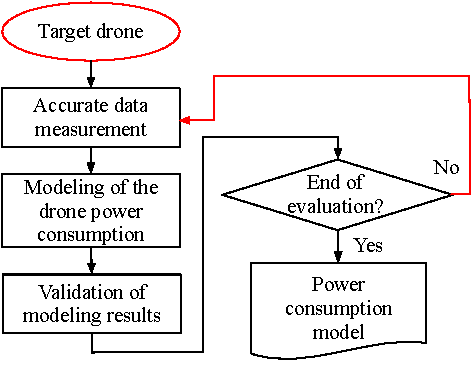
\includegraphics[scale= 0.85]{fig16/sub_problem_1.pdf}}
}
\label{fig:freamwork_a}
\qquad

\subfloat[
Sub-problem 2: Finding the minimum energy consumption path of the drone in a given mission.
]{
\fcolorbox{red}{white}{
    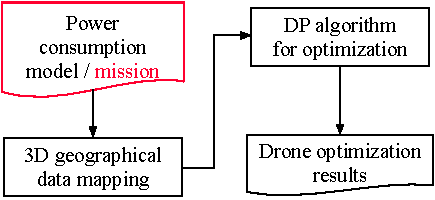
\includegraphics[scale= 0.91]{fig16/sub_problem_2.pdf}}
}
\caption{The systematic framework \textcolor{red}{for} the \textcolor{red}{least energy path planning of the} drone.}
\label{fig:freamwork_b}

\label{fig:freamwork}
\end{figure}









\section{Accurate drone power measurement}
\label{Section: Challenges in drone power measurement}



\subsection{Inaccurate data from \textcolor{red}{the} genuine flight computer}

Top-of-the-line commercial drones provide \textcolor{red}{information to the user about flight statuses}. 
We use the DJI Matrice 600 Pro (M600), which is a flagship model of DJI\,\cite{ref_11}, one of the world-leading drone companies. 
\textcolor{red}{The M600 is equipped with an A3 flight control module that includes an onboard measurement circuit storing the flight data at the sampling rate of 200 Hz.} 
However, the factory onboard measurement circuit is not accurate enough to build a power model. 
It goes without saying that the flight data should be accurate to build a useful power consumption model.
\textcolor{red}{In order to show the inaccuracy of the onboard measurement module, we compare the logged data from the onboard flight control module and a high precision data acquisition device (NI DAQ)\,\cite{ref_12} on the ground.}

\begin{table}[ht]
\caption{\textcolor{red}{The logged power consumption data from the genuine flight module of M600 without turning on the propulsion.}}
\label{Table: motor_status}
\resizebox{0.485\textwidth}{!}{%
\begin{tabular}{|c|c|c|c|c|c|c|}
\hline
Motor number & Motor 1 & Motor 2 & Motor 3 & Motor 4 & Motor 5 & Motor 6 \\ \hline
Voltage (V)  & 51.3 & 51.1 & 51 & 51.5 & 51.4 & 51.1 \\ \hline
Current (A)  & -0.05 & -0.57 & -0.15 & 0.19 & 0 & 0.45 \\ \hline
Power (W)    & -2.56 & -29.12 & -7.65 & 9.78 & 0 & 22.99 \\ \hline
\end{tabular}%
}
\end{table}

\noindent\textcolor{red}{We tightly secure the drone on the ground while we increase the throttle to make propulsion force.}
The measured \textcolor{red}{values in Table\,\ref{Table: motor_status} show} non-negligible negative current values that explain that there is a distinct DC offset in the \textcolor{red}{onboard} power measurement circuit.
%\textcolor{red}{We also check the accuracy of the logged power consumption while the drone is in the air. We tightly secure the drone on the ground while we increase the throttle to make propulsion force.}


\begin{figure}[ht]
\centering
\subfloat[The power measurement test on the ground.]{\includegraphics[scale= 0.80]{fig1/Ground_test.pdf}}
\qquad
\subfloat[\textcolor{red}{The measured current flow comparison between the NI DAQ and the onboard flight module.}]{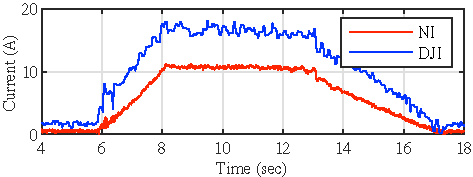
\includegraphics[scale=1.0]{fig1/NIvsDJI.pdf}}
\caption{\textcolor{red}{The experiment set to confirm the DC offset and the DC offset comparison result.}}
\label{fig:Ground_test}
\end{figure}

We configure the experiment environment for measuring the current using the shunt resistor and the operational amplifier (OP-AMP) as Fig.\,\ref{fig:Ground_test}(a)\textcolor{red}{.} \textcolor{red}{T}he experiment result is presented in Fig.\,\ref{fig:Ground_test}(b). 
It visualizes that the current profile of the factory onboard power measurement circuit is marginally \textcolor{red}{similar to the high precision data acquisition device,} but the actual scale is significantly different. 
In order to overcome this difference \textcolor{red}{and use the data from the onboard flight controller}, we attempt various trials by post-processing (calibration, etc.). 
However, the source of error \textcolor{red}{are} not only the DC bias and gain error but also \textcolor{red}{the} uneven sampling rate and lack of linearity. 
\textcolor{red}{Consequently,} we conclude that the \textcolor{red}{data from the} factory onboard \textcolor{red}{flight controller of} the drone is not appropriate for the research that we aim at because of \textcolor{red}{its inaccuracy}.




\subsection{Design of the \textcolor{red}{accurate} power measurement \textcolor{red}{system}}

\begin{comment}
\begin{figure}[ht]
\centering
\subfloat[The front of the circuit board.]{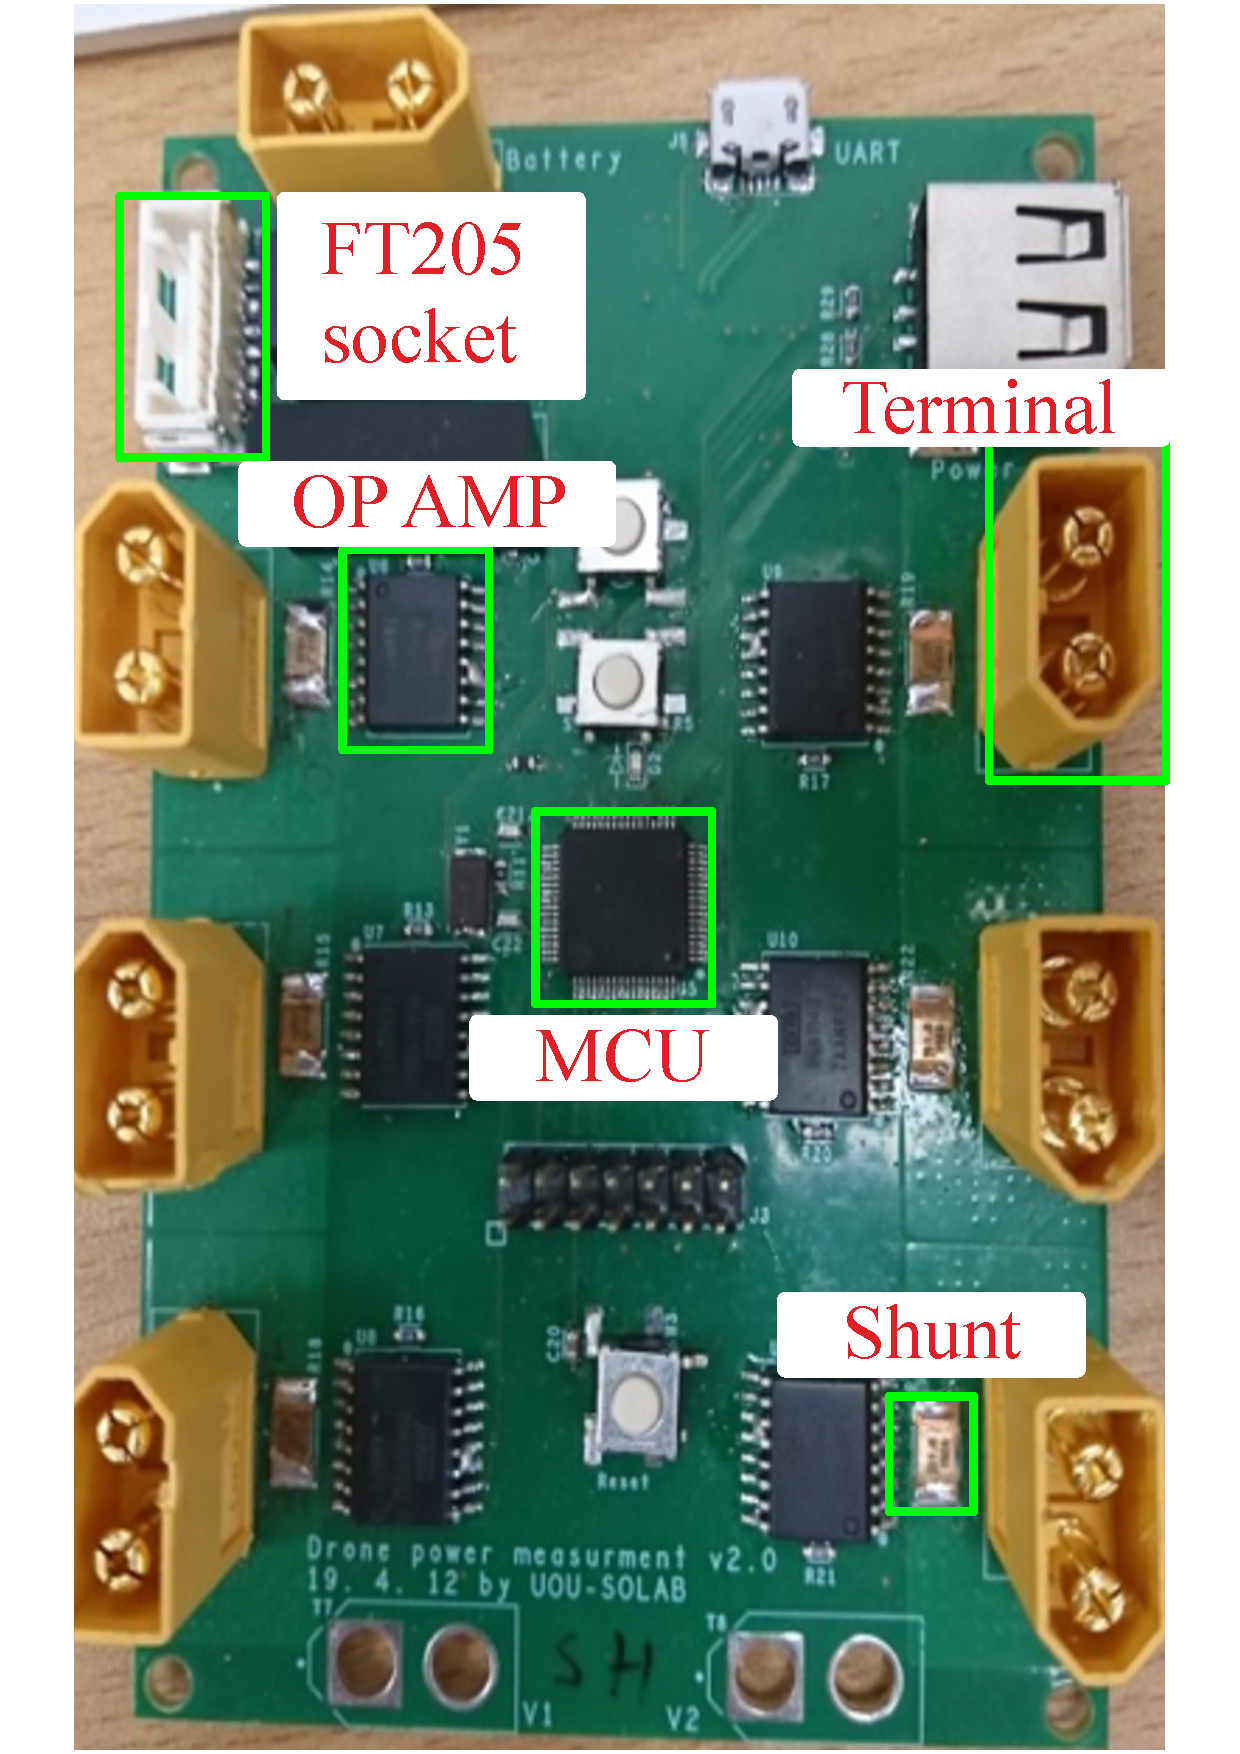
\includegraphics[scale=0.20]{fig2/New_board_front.pdf}}
\subfloat[The back of the circuit board.]{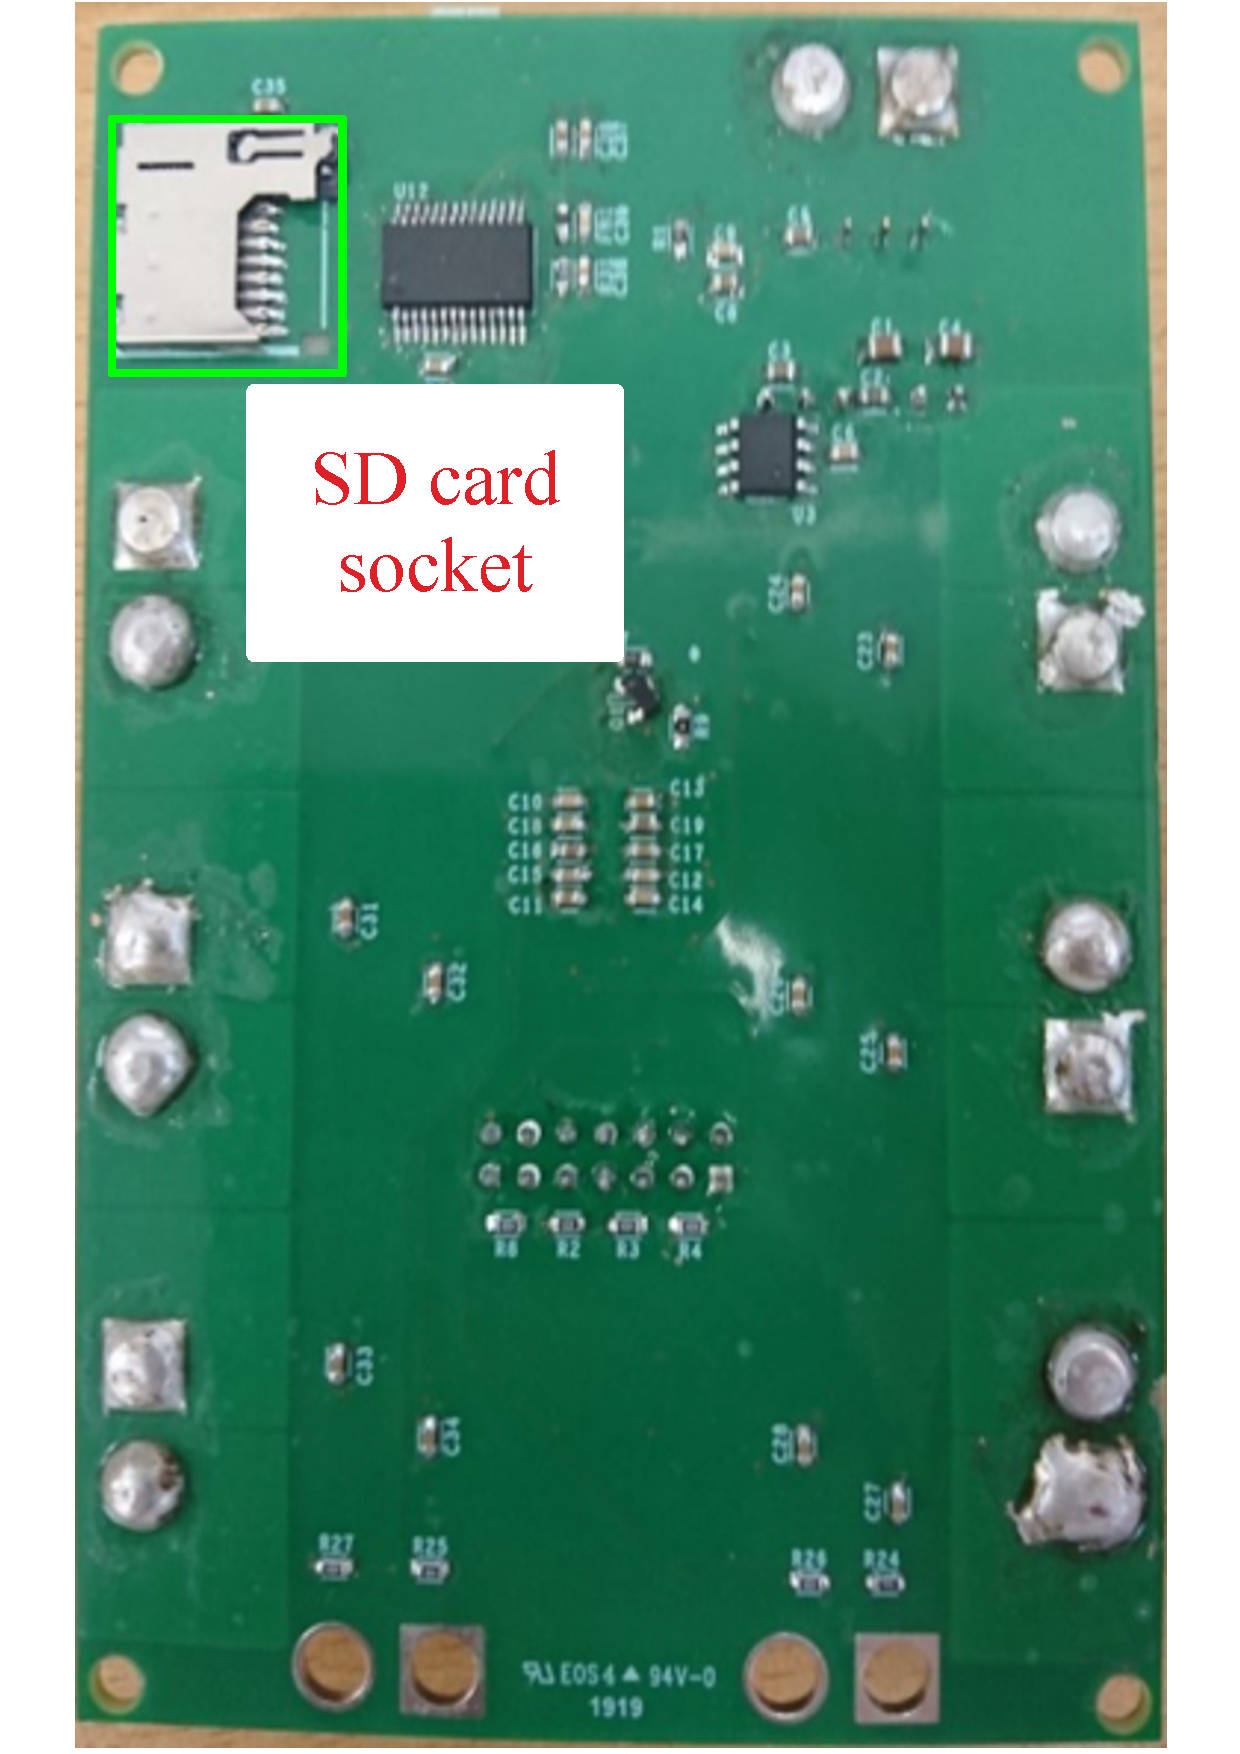
\includegraphics[scale=0.20]{fig2/New_board_back.pdf}}
\caption{The power measurement board installed on the drone.}
\label{fig:board}
\end{figure}
\end{comment}

We design the power measurement \textcolor{red}{system with} very high accuracy, like the high precision data acquisition device.
\textcolor{red}{We carefully select composing devices to ensure accuracy according to the specifications of the drone.
The power measurement system measures the voltage of the drone through voltage divider circuits that convert the drone operating battery voltage to the voltage that I/O of the microcontroller unit (MCU) can accept.  
It also acquires the current of the drone using the one milliohm shunt resistor and the amplifier.
The power measurement system is lightweight and separated battery-powered, so it does not affect the power consumption of the drone.
We use the real-time operating system (RTOS) on an MCU to ensure data sampling rate.
All measurement tasks store data at a sampling rate of 1~kHz.
The measured voltage and current values are periodically stored to the SD card as the binary format file that is readily processed externally.} 


\begin{figure}[ht]
\centering
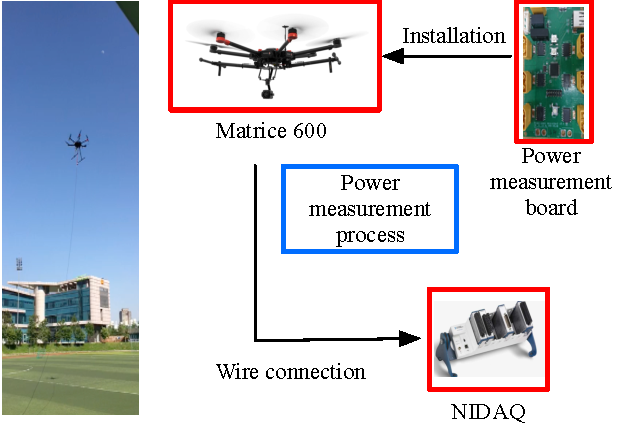
\includegraphics[scale=0.825]{fig3/flight_experiment.pdf}
\caption{The power measurement test during flight.}
\label{fig:flight_test}
\end{figure}

\begin{figure}[ht]
\centering
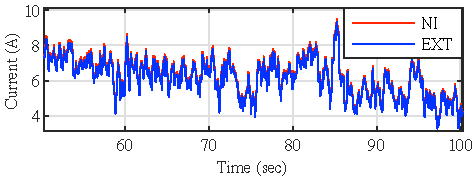
\includegraphics[scale=1.0]{fig4/flight_exp_result.pdf}
\caption{Comparison of the current measurement by each measurement device. The power measurement \textcolor{red}{system} presents data as accurate as NI DAQ.}
\label{fig:flight_result}
\end{figure}

\noindent\textcolor{red}{We measure the power consumption of the drone during the flight as Fig.\,\ref{fig:flight_test}. The measured power consumption overtime during the flight is depicted in Fig.\,\ref{fig:flight_result}.}
The measured current value on the power measurement \textcolor{red}{system} has an root mean square error (RMSE) of less than 6\,\% compared with the measured value with \textcolor{red}{the} NI DAQ. 
\textcolor{red}{Therefore, we collect power data using our precise power measurement system instead of the inaccurate factory onboard flight controller for the accurate power consumption model.}

\label{Section: Design the power measurement board}





\subsection{\textcolor{red}{Real-time kinetic global navigation satellite system}}
%The commercial drones always record their physical parameters such as velocity, acceleration to the backlog to confirm their flight status. 
\textcolor{red}{In general, drones determine their position through the inertial measurement unit (IMU) and Global Positioning System (GPS) modules. 
However, according to the manufacturer, the factory onboard GPS module on the M600 has a vertical error of 0.5 m and a horizontal error of 1.5 m, respectively. 
Such positional errors of the onboard genuine flight controller reduce the accuracy of the power consumption model even we use the accurate power measurement system.}
%When we synchronize the onboard genuine flight controller in the M600 and our power measurement system to use parameters as input variables of the power consumption model, 
\textcolor{red}{The real-time kinetic global navigation satellite system (RTK GNSS)} was developed for enhancing the accuracy of \textcolor{red}{the} commercial GPS.
Under the assistance of \textcolor{red}{the} ground GPS station, \textcolor{red}{the} RTK GNSS enhances the GPS accuracy to reduce the error to \textcolor{red}{within 10 cm}\,\cite{ref_13}.
We install \textcolor{red}{antennas of the} RTK GNSS on the drone and validate the improved accuracy by comparing it with another separate industrial high precision GPS module ATK980R\,\cite{ref_14}.
We conduct the following simple comparison for checking the performance of \textcolor{red}{the} GPS improved by \textcolor{red}{the} RTK GNSS.
First, we collocate the antennas of \textcolor{red}{the} ATK980R and the \textcolor{red}{M600} in the same position. 
\textcolor{red}{After that, we shift the ATK980R and the M600 into the same distance from the original position and compare the difference of GPS coordinates between two GPS modules.}
As a result of the comparison, \textcolor{red}{we confirm that the improved GPS module of the drone has less than 5~cm error by comparing it with the industrial GPS module.}
This error is about 20 times \textcolor{red}{less} than the error of the drone onboard GPS module.




\subsection{Wind sensor}

On the other hand, the wind profoundly affects the power consumption of drones as well as the other parameters \textcolor{red}{(e.g., velocity, acceleration).}
\textcolor{red}{Even if the drone is flying at the same velocity, the power consumption is changed by the wind velocity.}
This phenomenon becomes more severe \textcolor{red}{when} the overall surface area of the drone increases.
\textcolor{red}{However, it is challenging to measure wind and change the drone's path while the drone is working for the mission in real-time. First, the drone needs to equip the professional device to measure wind during the mission. And second, with the limited computing power of the drones flight controller, the wind of candidate paths cannot be predicted online.
Moreover, the wind gradient phenomenon, which varies the strength of the wind depending on the altitude, makes it difficult to analyze the influence of wind on drones flying at various altitudes\,\cite{ref_28}.
So, many studies conduct experiments using artificial wind or wind information of the region where the drone is flying provided by the national meteorological agency\,\cite{ref_5,ref_9}.
}
In this work, we measure the actual wind that affects the power consumption of drones \textcolor{red}{only to build the drone's power model}.
\textcolor{red}{We attach a wind sensor FT205 on the drone as Fig.\,\ref{fig:wind_sensor}\,\cite{ref_15}.}

\begin{figure}[ht]
\centering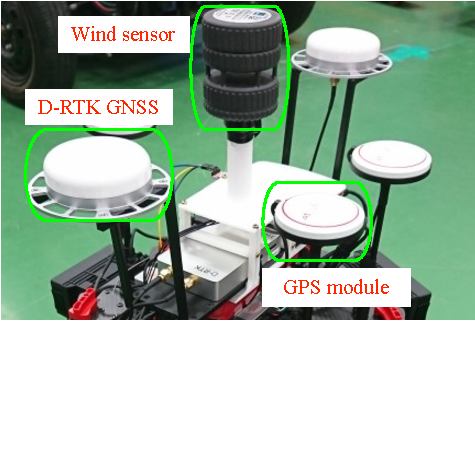
\includegraphics[scale=0.90]{fig5/wind_sensor_resize.pdf}
\caption{The picture of installed DJI's RTK GNSS and external wind sensor FT-205.}
\label{fig:wind_sensor}
\end{figure}

\noindent This sensor measures \textcolor{red}{the wind velocity of 360 degrees in the horizontal direction and has} a sampling rate of 10\,Hz and a maximum error of 0.3\,m/s.
\textcolor{red}{The sensor transfers the measured data to our power measurement system via UART communication, and the MCU of the power measurement system stores the wind data with power measurement data on the SD card under the control of the RTOS.
However, since the wind sensor can only measure wind in a horizontal direction, we cannot consider the vertical direction of the wind as a factor in the power consumption model.
Therefore, we assume that the influence of pure vertical wind to the drone is excluded, and we also assume that wind effects in the vertical direction are minimal above a certain altitude because we operate a drone at altitudes between 30 and 100 meters that are quite far from the ground.}









\subsection{Weight and volume of \textcolor{red}{the} payload}
\label{sub_section:lift}
As the total weight of a drone increases, \textcolor{red}{a drone demands more power for its thrust.
The wind resistance caused by the surface area also affects the power consumption of the drone when the drone delivers a payload.
Therefore, we collect data by varying the surface area and weight of payloads to confirm the influence of increased weight and surface area on the power consumption of the drone.
Helicopter effective translational lift, commonly called translational lift in the aerodynamics, always occurs when the rotor blades move horizontally.
The translational lift increases the lifting force by decreasing the induced drag of the drone when the rotor-craft moves at a certain velocity, no vortices occur in the rotor-craft, and the airflow is horizontal.
This additional lift at a certain velocity is called the effective translational lift (ETL), and its characteristic is affected by the features of the drone (e.g., weight, surface area, etc.).
To operate the aircraft at maximum performance, the ETL should be exploited\,\cite{ref_20}.
%The ETL is used when operating the aircraft at maximum performance\,\cite{ref_20}.
However, because too heavy payloads are very inefficient to be transported by drones, we set the weight limit up to\,2~kg, which is about a half of the maximum payload weight that the M600 can carry.
Based on the collected data, we present the velocity range in which the M600 can efficiently utilize energy under the ETL as shown in Fig.\,\ref{fig: lift}. 
}


\begin{figure}[ht]
\fcolorbox{red}{white}{
\centering\includegraphics[scale=1.0]{fig10/wind_lift.pdf}
}
\caption{The effect of the translational lift on the optimal velocity for the least energy consumption per meter.}
\label{fig: lift}
\end{figure}


The green line\textcolor{red}{, which is a baseline} in Fig.\,\ref{fig: lift}, \textcolor{red}{means} the energy consumed per distance versus the constant velocity of the drone without any payload when the wind sensor records the \textcolor{red}{neglectable} wind speed.
The red line \textcolor{red}{means} the energy consumed per distance versus the constant velocity of the drone with the payload of 2\,kg when the wind sensor records \textcolor{red}{the neglectable wind speed.}
The blue line \textcolor{red}{means} the energy consumed per distance versus the constant velocity of the drone without the payload when the wind sensor records the \textcolor{red}{intense} wind speed \textcolor{red}{(between 6\,m/s to 8\,m/s)} that \textcolor{red}{can affect} the power consumption of the drone.
\textcolor{red}{The blue line shows that the total power consumption of the drone increases when an overall surface increases. In this case, the drag force received by the drone increases, and the optimal velocity of the drone affected by the translational lift decreases slightly.}
On the other hand, when the weight is added, the total power consumption and the optimal velocity of the drone dramatically increases \textcolor{red}{like the red line.}
As the above results, the drone has various optimum flight velocity according to the \textcolor{red}{external} environment, and the optimal method of operating the drone can be determined by combining the optimum flight velocity and the battery consumption of the drone.

Note that when the weight is added to the drone, the velocity based on the translational lift exceeds the M600's safe \textcolor{red}{operation speed} range (up to 18\,m/s without the wind). Unavoidably, we \textcolor{red}{do not implement that case} in this paper due to a safety issue.








\section{Building a power consumption model of the drones}
\label{Section: Power consumption model for the drones}

As we mentioned in Section\,\ref{Section: Related works}, \textcolor{red}{the power consumption model of the} drones can be classified into \textcolor{red}{the dynamics model, the momentum theory model, or the data-driven model. 
However, in this work, we use the Deep neural networks (DNNs)}, one of the machine learning techniques, to build a model based on the power consumption data and other measurable parameters that affect the power consumption of the drone collected in Section\,\ref{Section: Challenges in drone power measurement}.
\textcolor{red}{The DNNs model uses} simple \textcolor{red}{variables} that can represent the motion of the drone instead of the theory-based formulas as in the conventional regression method. 
Besides, since \textcolor{red}{the DNNs} can theoretically approximate all \textcolor{red}{the} functions, it is possible to predict the complex power consumption process of drones well.
In this section, \textcolor{red}{we present the grid search results for constructing the optimal neural network structure and show the accuracy of the DNNs model through the six kinds of benchmark flights.
Then, we compare the model accuracy of the completed DNNs model and other theoretical models.}



\subsection{\textcolor{red}{Deep neural networks}}

The most frequently used methods \textcolor{red}{optimizing the hyper-parameters of the DNNs are the random search and the grid search method\,\cite{ref_16}.} 
\textcolor{red}{Among} them, we use the grid search method that obtains the best result \textcolor{red}{in the given conditions}, and then we record the performance metric as \textcolor{red}{the RMSE} for each hyper-parameter combination.
We search the number of hidden layers from 3 to 70 and the number of hidden neurons from 10 to 100. 
\textcolor{red}{During searching for the network structures, the learning rate gradually decays from 1e-2 to 1e-4, and the batch size changes from 64 to 4096 for each hyper-parameter combination.}
We \textcolor{red}{apply} the Rectified \textcolor{red}linear \textcolor{red}{u}nit (ReLU) and the linear function as \textcolor{red}{the activation function} for the hidden layers and the output layer, respectively.
Also, \textcolor{red}{we select the Adaptive moment estimation (ADAM) and Stochastic gradient descent (SGD) optimizer as the candidate for the learning algorithms\,\cite{ref_17}. 
The input variables of the network consist of the three-axis velocity and acceleration, altitude, two-axis wind velocity, and the weight and surface area of loads.} 
\textcolor{red}{We randomly exclude 0.5\,\% of the 30 hours flight data to validate the trained model, and use the remaining data as the training data.
The grid search takes 370 hours under the Intel\textregistered \,i7-8086K CPU @ 4.00\,GHz (12 cores) and NVIDIA\textregistered \,GeForce 1080Ti 16\,GB. 
As a grid search result, we use the DNNs power consumption model with} the learning rate of 0.0005, 44 neurons, 35 hidden layers, 2048 batch size, ReLU for the activation function, and ADAM for the learning algorithm.
\textcolor{red}{Once we found the optimal neural network structure, we do not repeat the grid search unless there is a change in the input variables of the power consumption model.
It takes about 10\,minutes to train the power consumption model through the optimal network structure and actual flight data of 30\,hours.}

\begin{comment}
\begin{table*}[ht]
\caption{The list of grid search results}
\label{Table: gridsearch_result}
%\resizebox{0.485\textwidth}{!}{%
\centering
\begin{tabular}{|c|c|c|c|c|c|l|}
\hline
 & Epoch & Learning late & Neurons & Hidden layers & Batch size & Optimizer \\ \hline
\textcolor{red}{1} & 690   & 0.0005  & 44 & 35 & 2048 & \hspace{0.05cm} ADAM \\ \hline
\textcolor{red}{2} & 494   & 0.001   & 60 & 60 & 2048 & \hspace{0.05cm} ADAM \\ \hline
\textcolor{red}{3} & 277   & 0.0003  & 80 & 60 & 2048 & \hspace{0.05cm} ADAM \\ \hline
\textcolor{red}{4} & 794   & 0.0002  & 44 & 35 & 4096 & \hspace{0.05cm} ADAM \\ \hline
\textcolor{red}{5} & 709   & 0.001   & 44 & 30 & 512  & \hspace{0.05cm} ADAM \\ \hline
\textcolor{red}{6} & 844   & 0.005   & 36 & 25 & 4096 & \hspace{0.05cm} ADAM \\ \hline
\textcolor{red}{7} & 577   & 0.0005  & 36 & 35 & 512  & \hspace{0.05cm} ADAM \\ \hline
\end{tabular}%
%}
\end{table*}
\end{comment}

\label{Section: Deep Neural networks (DNN)}





\subsection{Validation of \textcolor{red}{the} power consumption model}

\textcolor{red}{The autonomous driving of the drone is much easier to adjust the velocity and acceleration required for the drone operation than the direct control by the user.
We implement the autonomous driving of the drone by using the software development kit (SDK) provided by DJI with the robot operating system (ROS), which is often used in the robotics field. 
In order to validate the accuracy of our power consumption model, we upload the six types of the autonomous driving path to the drone and perform the actual flight.}
\textcolor{red}{In Fig.\,\ref{fig: benchmark}, all figures show the measured power consumption from the drone and estimated power consumption from the DNNs model} when \textcolor{red}{(a)} the drone is hovering in the air, \textcolor{red}{(b)} the drone repeats vertical flights (ascending and descending without horizontal movement), \textcolor{red}{(c) the drone flies an interval path that repeats the straight flight and back straight flight without vertical movement}, \textcolor{red}{(d)} the drone is flying a \textcolor{red}{rectangular path}, and \textcolor{red}{(e)} the drone with the payload repeats straight flight of constant velocity, respectively. 
\textcolor{red}{When we compare the measured power consumption value with the predicted value of all the benchmark tests, the RMSE are (a) 6.27\,\%, (b) 9.8\,\%, (c) 7.82\,\%, (d) 9.12\,\%, and (e) 10.14\,\%, respectively.}

\begin{figure}[h]
\centering
\subfloat[Drone power consumption when hovering.]{\centering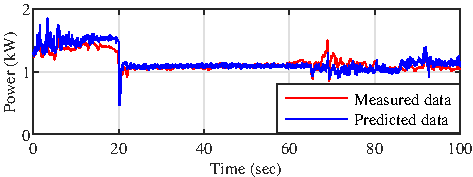
\includegraphics[scale=1.05]{fig8/Hover8x3.pdf}}
\qquad
\subfloat[Drone power consumption when ascending and descending.]{\centering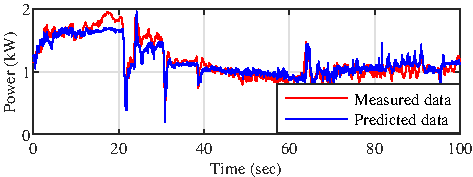
\includegraphics[scale=1.05]{fig8/AD8x3.pdf}}
\qquad
\subfloat[Drone power consumption when interval flight.]{\centering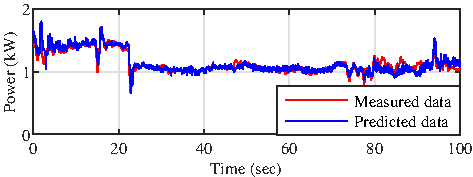
\includegraphics[scale=1.05]{fig8/Interval8x3.pdf}}
\qquad
\subfloat[Drone power consumption when squared-shaped flight.]{\centering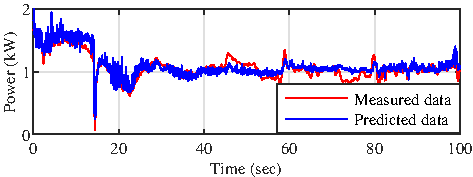
\includegraphics[scale=1.05]{fig8/Square8x3.pdf}}
\qquad 
\subfloat[\textcolor{red}{Drone power consumption} with payload and without payload during constant speed flight of 6\,m/s.]{\centering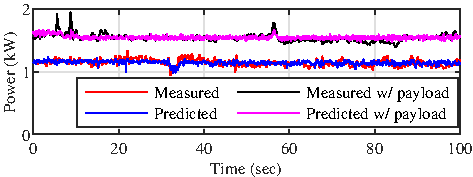
\includegraphics[scale=1.05]{fig9/compare_weight8x3.pdf}}

\caption{Comparison of measured power consumption and predicted power consumption under the benchmark flights.}

\label{fig: benchmark}
\end{figure}

\subsection{\textcolor{red}{Comparison of the power modeling methodologies}}

\textcolor{red}{Our proposed DNNs model consists of simple variables that represent simple drone movement and external forces. It does not require complex knowledge of the dynamics or control theory and has a high enough accuracy of about 90~\% compared with the actual flight data.}
\textcolor{red}{We present prediction results of the proposed DNNs model, the model using momentum theory\,\cite{ref_4}, the model using aerodynamics\,\cite{ref_3}, and the data-driven model using the linear regression in Table\,\ref{Table: power_modeling}~\cite{ref_8}.
As a result above, the DNNs model is the highest accuracy compared with other models.
However, predicting power consumption through neural networks is relatively slower than using numerical formulas, and the neural networks require a lot of effort to build the model through training: The DNNs model has a trade-off relationship between accuracy and speed.
Clearly, the DNNs model has an advantage in the accuracy, which is required when performing a large-scale search such as an optimal path planning rather than a real-time search that requires continuous fast power consumption prediction.
Therefore, we use the highest accurate model (DNNs) to predict the power consumption in each step of the process for optimizing drone operations.
We configure the power model of the drone so far, and we introduce the optimization of the minimum energy path of the drone using the power model configured in Section\,\ref{Section: Optimization} that follows.}

\begin{table}[ht]
\centering
\textcolor{red}{
\caption{Comparison of the result accuracy between power models}
\label{Table: power_modeling}
%\resizebox{0.38\textwidth}{!}{%
\fcolorbox{red}{white}{
\begin{tabular}{|c|c|}
\hline
{Power modeling method} &  {Error rate (\%)} \\ \hline
{Aerodynamics\,\cite{ref_3}}          & { 14.90}           \\ \hline
{Data-driven\,\cite{ref_8}}           & { 13.73}           \\ \hline
{Momentum theory + translocation term\,\cite{ref_4}}       & { 10.07}           \\ \hline
{Deep neural networks}  & { 9.27}            \\ \hline
\end{tabular}%
%}
}
}
\end{table}















\section{Flight energy optimization}
\label{Section: Optimization}

We predict the energy consumption when a drone \textcolor{red}{departs} from a starting point to a designated destination avoiding obstacles while flying downtown. 
After deriving a \textcolor{red}{minimum energy consumption flight path through the power consumption model and optimization algorithms}, we validate \textcolor{red}{the result by comparing predicted total energy consumption with measured energy consumption of actual flight.}
As we mentioned in Section\,\ref{Section: Related works}, there are advantages and disadvantages in \textcolor{red}{optimization methods for the drone through the numerical and graph search algorithms.}
The numerical algorithms are suitable for expressing the momentary movements of the drones. 
\textcolor{red}{But,} it is not ideal for calculating all the actions of the drone about half an hour at a wide range.
\textcolor{red}{Therefore, we use the graph search algorithm for our optimization to consider the overall operation of drones.
In this section, we formulate the optimization problem of the drone and define conditions for applying the optimization algorithm.
We also set up heuristics to overcome the weaknesses of the graph search algorithm, and then explain how the Dijkstra algorithm, one of the dynamic programming, applies to our problems.}




\subsection{\textcolor{red}{Problem formulation}}

\begin{figure}[ht]
\fcolorbox{red}{white}{
\centering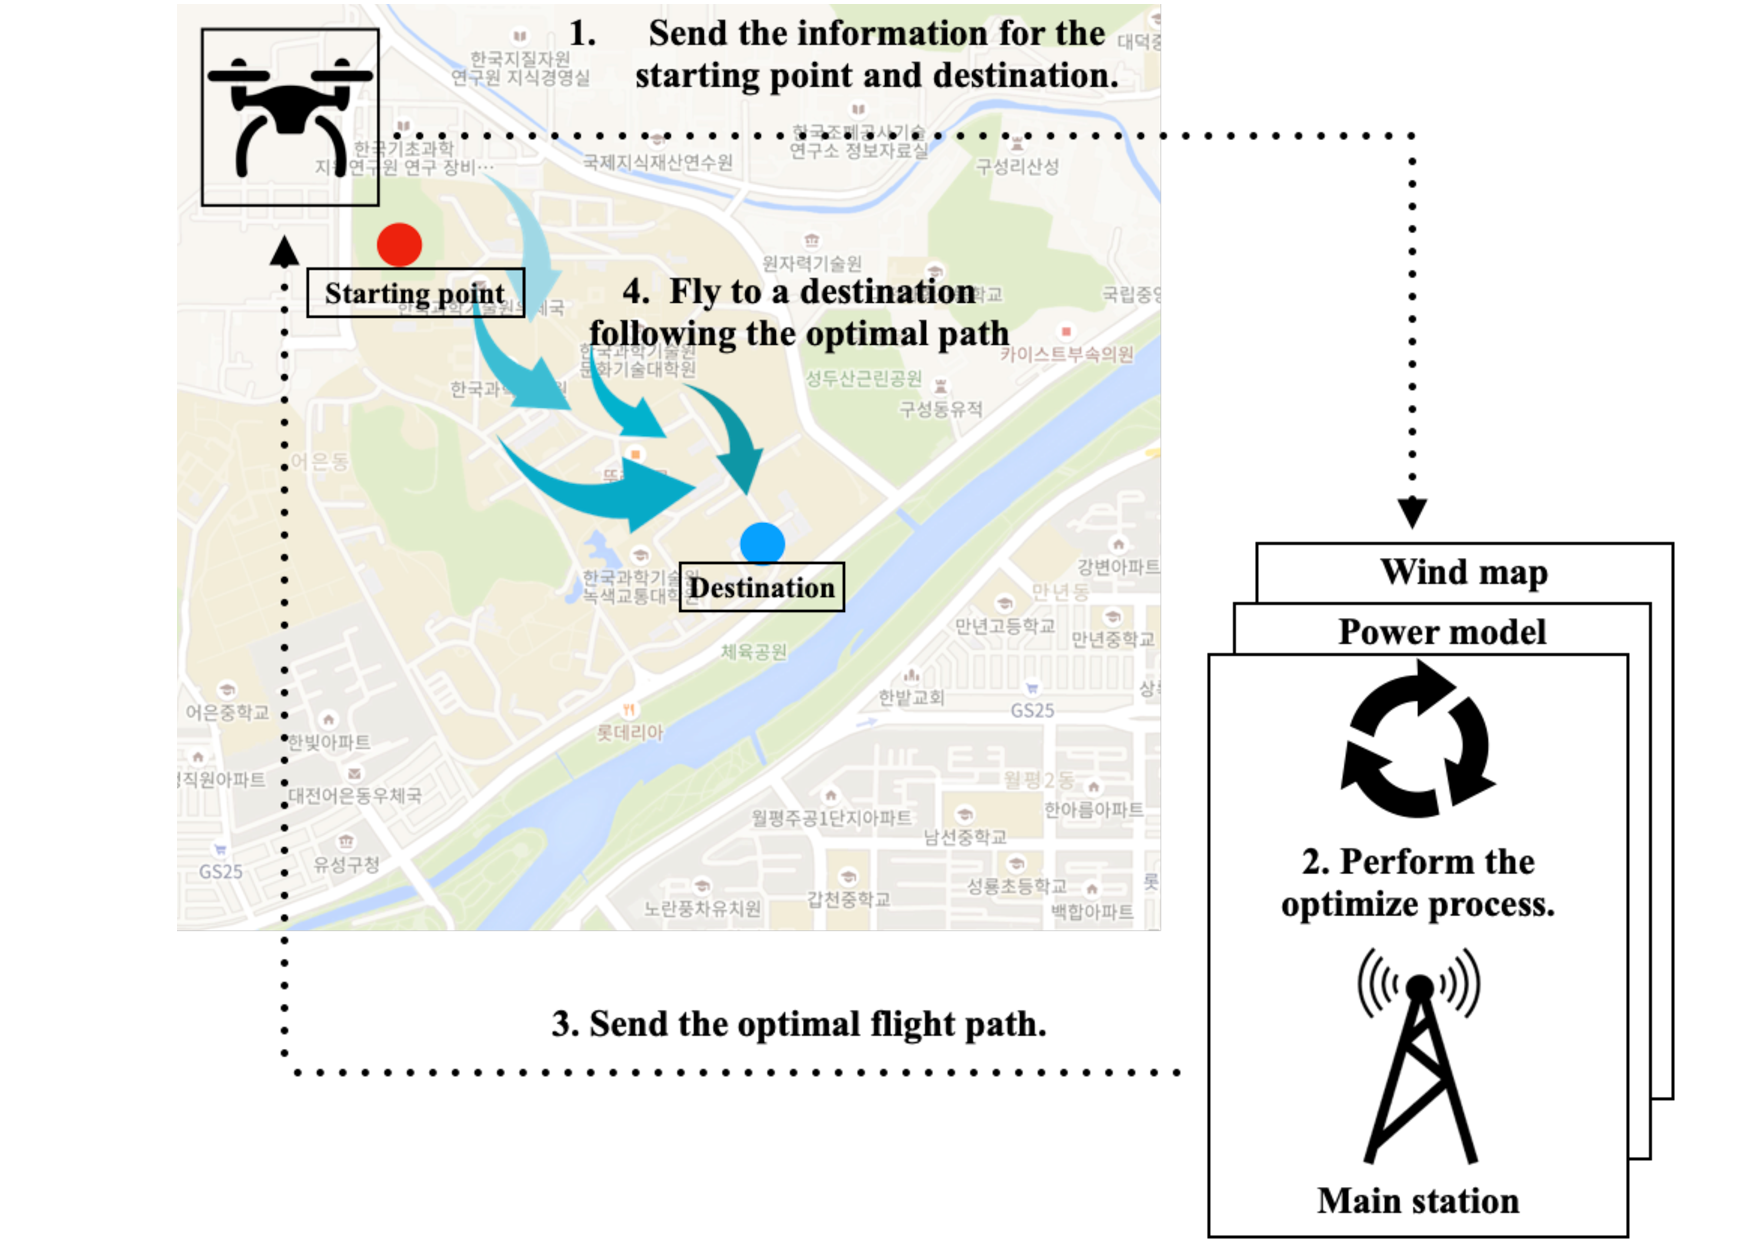
\includegraphics[scale=0.34]{fig17/problem_formulation.pdf}}
\caption{\textcolor{red}{The scenario of the drone optimization process.}}
\label{fig:problem_formulation}
\end{figure}

\textcolor{red}{In our scenario, the operator inputs information about a starting point and a destination to the main station to assign a task to the drone, as shown in Fig.\,\ref{fig:problem_formulation}.
The station holds the power consumption model of the drone and wind maps about the operating environment, and the station derives the path between points entered from the operator.
% Offline 최적화임을 여기서 언급
Since the optimization is performed offline at the main station, it is impossible to modify the optimal path already drawn while the drone is running. Also, in this paper, we do not assume that the station considers the unexpected situations such as bird-strike or wind-sheer.
% 외부 바람을 고려하기 위해 전용 툴을 쓴다는 것을 여기서 언급함
However, we analyze the predictable external forces such as wind level and direction using the sophisticated analysis tool to take full advantage of the effects of external forces in creating the optimal path of the drone. 
After that, the drone receives the optimized path from the station and then runs to the destination along the path. We formulate the flight energy optimization problem of the drone as the following:}

\textcolor{red}{
\vspace{7pt}
\hrule
\vspace{5pt}
\noindent\textit{\textbf{Flight energy optimization problem formulation}}
\vspace{5pt}
\hrule
\vspace{5pt}
\noindent Workspace $W$ is a subset of $\mathbb{R}^3$ that drones can maneuver, and $F(\cdot)$, $B(\cdot)$ take the $W$ as the domain:\\
\indent Workspace, \textit{$W\subset\mathbb{R}^3$, $w_n=(x_n,y_n,z_n)$, $w_n \in W$ }\\
\indent Blockage, \textit{$BL(w_n)=bl_n$}, while blockage $bl_n\in\{0,1\}$\\
\indent Wind field, \textit{$F(w_n) = (windx_n, windy_n)$}, while $windx_n$ is  
\indent x-axis wind velocity and $windy_n$ is y-axis wind velocity
\indent at $w_n$, respectively.
\vspace{5pt}
\hrule
\vspace{5pt}
\noindent\textit{\textbf{Given:}}~\\
\indent $W, F(\cdot), BL(\cdot)$~\\
\indent Set of delivery missions, $M = \{m_1, ..., m_J\},$~\\ 
\indent $m_j = (from, to, package\;volume, package\;weight)$~\\
\noindent\textit{\textbf{Control knob:}}~\\
\indent Path, finite sequence of $(w,v)$,~\\
\indent $R = \{(w_0,v_0), ..., (w_N,v_N)\}$, while $v$ is a velocity vector.
\noindent\textit{\textbf{Objective:}}~\\ 
\indent Minimize total consumption energy~\\
\indent\indent $\sum_{j=1}^J E(m_j,R_j)$,~\\
\indent while $E$ is energy consumption for the delivery mission $m_j$~\\
\indent through a path $R_j$, which satisfies~\\
\indent\indent $BL(w_n) = 0, \forall w_n \in \bigcup_{1}^J R_j,$~\\
\indent\indent $E(m_j, R_j) \leq$ Initial battery capacity.
\vspace{5pt}
\hrule
\vspace{5pt}
}
\vspace{5pt}

\textcolor{red}{In our optimization problem, the workspace $W$ where the drone is operated, the wind information $F$ in the horizontal directions provided through the discretized wind map, and the information of obstacles in the environment $BL$ are $Given$ information.
The starting point and destination of the mission, and information of the payload are also $Given$ information.
We define the function $Path$ using $w$ within the $W$ and the velocity of the drone $v$ as $R$, and we use the function $Path$ as our control knob.
Our objective is to find $Path$ that minimizes the function $E$ of the energy through the optimization process when a base station receives the mission $m$ from a drone.
The energy function $E$ cannot exceed the initial battery capacity, $BL$ must be zero for all $w$, and $Path$ consists only of $w$ presented in $W$.}






\subsection{Configuration of optimization \textcolor{red}{environments}}
\label{sub_Section: configuration}

We model the \textcolor{red}{discretized} operating environment of the drone as Fig.\,\ref{fig: opt_env}(a).
\textcolor{red}{We assume that there are various types of buildings in the environment, and the environment has the maximum range of 400\,m for the N- and E-axis and 80\,m for the U-axis, respectively.}
The drone in the environment can move \textcolor{red}{in} 10\,m for each step of horizontal axis and 3\,m for each step of vertical axis. \textcolor{red}{But}, the drone cannot pass through obstacles.
Besides, the drone moves in one direction per step by selecting a moving direction, \textcolor{red}{which is one of 26 directions from the current step to the next step as Fig.\,\ref{fig: opt_env}(b).}
However, when optimizing the flight path of the drone with one destination, the backward direction must be excluded because the drone consumes more energy as the \textcolor{red}{flight} time becomes longer. Therefore, we conclude \textcolor{red}{that} there are 17 \textcolor{red}{directions} for the drone to move on to the next step.
Previous studies using the graph search algorithm assume that \textcolor{red}{the drone} moves at a constant velocity between nodes because it is difficult to calculate \textcolor{red}{the continuous movement of the drone between discretized steps}\,\cite{ref_8, ref_10, ref_22}. 
On the other hand, we set the range of the drone velocity from a minimum of 6\,m/s to a maximum of 15\,m/s to explain the power consumption changing by the velocity change. 
\textcolor{red}{The range of velocity is determined based on each case of the least energy-consuming velocity of the translational lift effect in Fig.\,\ref{fig: lift} of the drone environment.}
At the same time, we take into account the effect of the drone acceleration that significantly affects \textcolor{red}{its power consumption.
We discuss the problem that arises when considering the acceleration of the drone on the optimization and define heuristics that is applied to solve the problem.}


\begin{figure}[ht]
\centering
\fcolorbox{red}{white}{
\subfloat[The isometric view of the \textcolor{red}{visualized} environment \textcolor{red}{where} drones fly \textcolor{red}{in}.]{\centering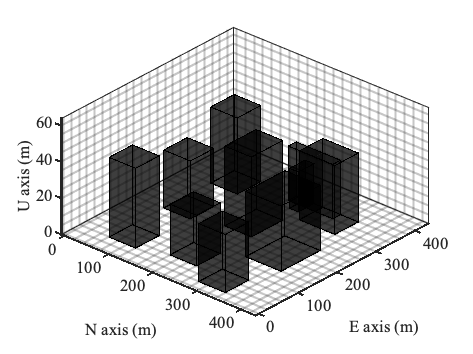
\includegraphics[scale=0.55]{fig11/obs.pdf}}
\hspace{4pt}
\subfloat[The \textcolor{red}{possible} direction \textcolor{red}{of} the drone.]{\centering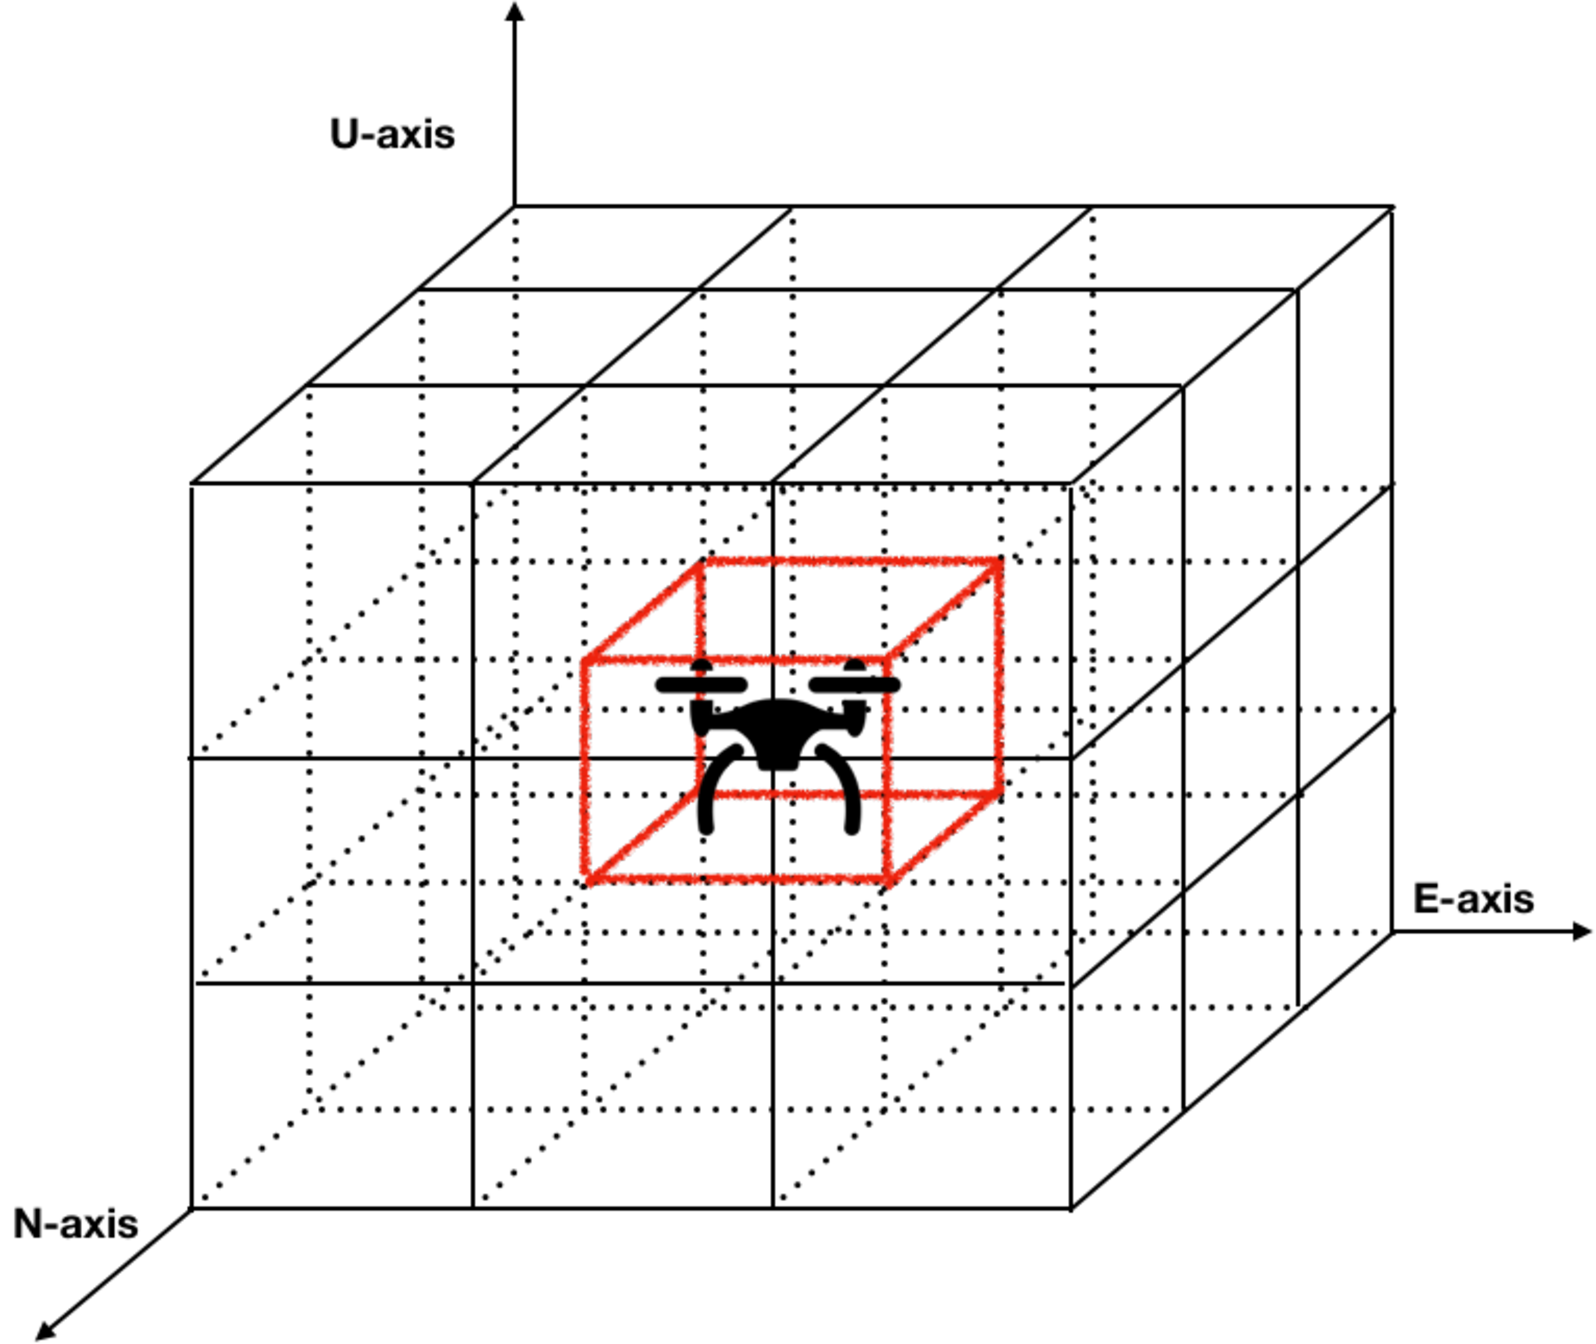
\includegraphics[scale=0.150]{fig11/Direction.pdf}}}
\caption{Visualization of the drone operating environment and the drone moving direction within the environment.}
\label{fig: opt_env}
\end{figure}

\textcolor{red}{We construct the graph from the referred three-dimensional space with the assumption of no influence of the radius of curvature of the earth.
%In general, a graph means a data structure composed of nodes and edges, and all connection data between nodes of the graph is stored in a binary adjacency matrix or edge list for searching the graph.
We set the parameters of the drone and the factor of the operating environment as a node.
%The node contains the parameters of the drone and the factors of the operating environment.
We notate each axis position information of the drone at the node i as $x_i$, $y_i$, and $z_i$, and also, we define the velocity and acceleration of the drone to $v_i$ and $a_i$, vice versa.
The wind speed and direction are denoted as $w_i$ and $d_i$. 
Note that the weight and surface area increase when a load is added on the drone. But they are constant values when a given mission. The acceleration of the drone $a_i$ can be inferred lately through Algorithm 1.}
Therefore, the node $n_i$ is declared as 
\begin{equation*}
n_i = (x_i, y_i, z_i, v_i, a_i, w_i, d_i). \tag{6.1} \label{eq:node}
\end{equation*}
%여기까지 노드.

%고다음부터는 edge.

\noindent\textcolor{red}{On the order hand, the edge is the path that can be moved between the nodes. It has energy consumption between connected two-node as edge weight.}
The edge weight \textcolor{red}{as} the energy consumption \textcolor{red}{is} calculated by combining the time required for the \textcolor{red}{traveling between two nodes} and the average instantaneous power consumption of each node, which can be expressed following that: 

\begin{equation*}
E(n_j, n_k) = \frac{P(n_j)+P(n_k)}{2} \Delta t, \tag{6.2} \label{eq:edge}
\end{equation*}
where $P(n_j)$ and $P(n_k)$ are the instantaneous power at the $n_j$ and $n_k$, and $\Delta t$ is the time taken to move \textcolor{red}{along the edge between the nodes}.

\textcolor{red}{
%The wind velocity is a crucial factor that significantly affects the power consumption of the drone, but it is difficult to grasp the influence of the wind on the power consumption of the drone because it needs to measure them directly in real-time. 
%위 얘기 wind -sensor 파트에서 이미 얘기했음.
The wind velocity is a crucial factor that significantly affects the power consumption of the drone. Let us assume that the wind is measured with a dedicated expensive sensor by the drone in real-time. There would be a long process occurs; 
the drone measures the wind for each step, transmits the information to a station far away, and transmits the movement corresponding to the next step derived from the station back to the drone.
During the process, the time lag generated by the calculation time for optimization in each step affects the optimal operation of the drone. 
Also, long-distance communication between the drone and station also consumes the computational and power cost of the drone.
Unless the user measures wind directly from the drone, there are very limited methods for obtaining wind information (for example, receiving the data from the meteorological agency).
In order to overcome these difficult conditions, we use a method to create a wind map through the CFD so that we can consider the effects of wind on drones in offline optimization.
Computational fluid dynamics (CFD) uses computers to simulate the interaction of fluids and gases in engineering problems\,\cite{ref_26}. 
The CFD converts the Navier-Stokes Equations, which are nonlinear partial differential equations describing fluid phenomena, into algebraic equations, and solves and analyzes fluid flow problems using algorithms of numerical techniques.
We build wind map from the average wind speed data provided by the meteorological agency for the drone operation through the flow analysis using the CFD and store them for each wind speed wind direction, as shown in Fig.\,\ref{fig: wind_map}(a).}

\begin{figure}[ht]
\centering
\fcolorbox{red}{white}{
\subfloat[\textcolor{red}{The flow analysis through the CFD.}]{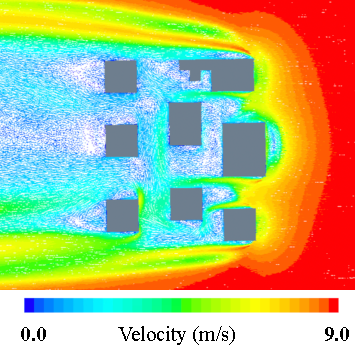
\includegraphics[scale=0.55]{fig18/CFD_map.pdf}}
\hspace{5pt}
\subfloat[\textcolor{red}{The discretized wind map converted from the flow analysis of the CFD.}]{\includegraphics[scale=0.57]{fig15/wind_N.pdf}}}
\caption{\textcolor{red}{The wind map configuration for the optimization environment.}}
\label{fig: wind_map}
\end{figure}

\noindent\textcolor{red}{
%However, since the power consumption model only includes the horizontal wind velocity directly measured by the wind sensor attached to the drone, we assume that the effect of the wind at pure vertical speeds on the drone is excluded, as mentioned in Section IV.
We only use the horizontal wind velocity analyzed through CFD at each step of the height axis except for the influence of the pure vertical wind since the drone power consumption model only includes the horizontal wind velocity, which is directly measured by the wind sensor attached to the drone. 
We assume that the effect of the pure vertical wind on the drone is excluded as mentioned in Section IV.
We convert the analyzed wind data through CFD to the discretized wind map like Fig.10(b) and make it possible to match the three-dimensional coordinate information of the graph with the wind velocity of the discretized wind map.
%The wind map contains the flow phenomena that occur when each direction of the wind from the inlet to an intensity of 9 m/s meets obstacles.
We build various wind maps by changing inlet wind directions.}
After that, \textcolor{red}{we use wind maps} as a lookup table so that the optimal route of the drone could be searched offline without \textcolor{red}{measuring} the wind directly from the drone.







\subsection{\textcolor{red}{Algorithm} to \textcolor{red}{calculate traveling time} between each node} % \textcolor{red}{considering acceleration} }
\label{sub_Section: Graph search}


In contrast to the studies using the conventional graph search algorithms that use the heuristics, \textcolor{red}{which exclude} the velocity change to reduce the \textcolor{red}{graph} dimension, we include the drone acceleration that significantly affects its power consumption.
Therefore, we \textcolor{red}{define an} algorithm to consider acceleration \textcolor{red}{of the traveling} between each unit node. 
%노드를 이동하는 드론의 가속 혹은 감속의 시간이 얼마나 되는지, 혹은 드론이 가속 또는 감속을 할때 드론이 다음 노드의 위치에 정확하게 도달할 수 있게 드론의 이동에 대한 휴리스틱을 고안한다.
We devise heuristics about the drone movement to solve \textcolor{red}{how much time is spent to accelerate or decelerate between nodes and how to make the drone accurately reach the position of the next node.
%We devise heuristics about the drone movement to solve how much to accelerate or decelerate the drone while moving between nodes, and how to make the drone reach the position of the next node accurately, considering the difference in moving distance generated by proceeding the acceleration or deceleration of the drone.
The following heuristics are based on assumptions that the drone must meet when moving between nodes:}

\begin{itemize}
\item Heuristic 1. \textcolor{red}{About t}he distance and travel time between the current node and the next node: \textcolor{red}{Even if each distance in the three-axis direction is different, we enforce that traveling time in the three-axis is all the same so the drone accurately moves from the previous node to the next node.}
\begin{comment}
  \begin{itemize}
      \item\textcolor{red}{When the moving direction of the drone at the current node is different from the next node, the difference of travel distance is caused by the acceleration or deceleration of the drone to the target velocity.}
      \item\textcolor{red}{The current node remembers the moving direction and velocity information of the drone at the previous node to consider the travel distance and time changes by the acceleration or deceleration.}
      \item \textcolor{red}{Even if each distance in the three-axis direction is different, we enforce that traveling time is all the same so the drone accurately moves from the previous node to the next node.}
  \end{itemize}
\end{comment}
\item Heuristic 2. \textcolor{red}{About t}he instantaneous velocity at the next node: \textcolor{red}{During the traveling, the drone first accelerates to the target velocity if it is necessary. Then, it moves the remaining distance with constant velocity. In case of the deceleration, the drone moves constant velocity. Then it decelerates to the target velocity lastly.}
\begin{comment}
  \begin{itemize}
      \item The drone from the current node to the next node must reach the velocity specified in the next node by either acceleration or deceleration.
      \item \textcolor{red}{The drone accelerates to the target velocity of the next node and then moves the remaining distance with uniform velocity.}
  \end{itemize}
\end{comment}
\end{itemize}

\SetNlSty{}{\color{red}}{:}
\SetAlFnt{\color{red}}
\begin{algorithm}[htp]
\caption{Finding $\Delta t$, which is the travel time between node $n_c$ and $n_n$.}
\SetAlgoLined
\KwInput{ \\
\hskip1.5em $G$ // The graph \\
\hskip1.5em $V_c$, $V_n$ // The velocity of the current and next node \\
\hskip1.5em $V_c$ := $(V_c[N], V_c[E], V_c[D])$ \\
\hskip1.5em $V_n$ := $(V_n[N], V_n[E], V_n[D])$ \\
\hskip1.5em $A_h, A_v$ // The maximum accelerations of the drone \\
\hskip1.5em $d$ // The distance between $n_c$ and $n_n$ \\
\hskip1.5em $d$ := $(d[N], d[E], d[D])$
}
\KwOutput{ \\
\hskip1.5em $\Delta t$ // The longest travel time between $n_c$ and $n_n$
}
\nonl \hrulefill \\
$\Delta t$ := $(\Delta t[N], \Delta t[E], \Delta t[D])$ \\
Initialize the $\Delta t$ \\
\For {$axis \in \{N,E,D\}$ \normalfont{between} $V_c$ \normalfont{and} $V_n$ \normalfont{in} $G$}
{
\If {$V_n[axis], V_c[axis] := 0$}
{
$\Delta t[axis] = \infty $
 }
\ElseIf {$V_n[axis] \ne 0$}
{ \begin{equation*}
\small{ \Delta t_1 :=
\begin{cases}
\cfrac{V_n[axis] - V_c[axis]}{A_h},~\text{if $axis = x,y$}\\
\cfrac{V_n[axis] - V_c[axis]}{A_v},~\text{else}\\
\end{cases}
}
\end{equation*}
\If {$d[axis] = \Delta t_1 \times {\abs{V_n[axis] + V_c[axis]}}\div{2}$}
{
    $\Delta t_2 := 0$
}
\Else
{
    $\Delta t_2 := \cfrac{(d[axis] - \Delta t_1 \times \cfrac{\abs{V_n[axis] + V_c[axis]}}{2})}{\abs{V_n[axis]}}$
}
}
\Else
{
\begin{equation*}
\small{
\Delta t_1 := 
\begin{cases}
\cfrac{V_n[axis] - V_c[axis]}{A_h},~\text{if $axis = x,y$}\\
\cfrac{V_n[axis] - V_c[axis]}{A_v},~\text{else}\\
\end{cases}
}
\end{equation*}
\If {($d = \Delta t_1 \times  {\abs{V_n[axis] + V_c[axis]}} \div {2}$)}
{
    $\Delta t_2 := 0$
}
\Else
{
        $\Delta t_2 := \cfrac{(d[axis] - \Delta t_1 \times \cfrac{\abs{V_n[axis] + V_c[axis]}}{2})}{\abs{V_c[axis]}}$
}
}
  $\Delta t[axis] = \Delta t_1 + \Delta t_2$
}
\Return $\Delta t = max(\Delta t)$ 
\end{algorithm}
\SetNlSty{}{\color{black}}{:}
\SetAlFnt{\color{black}}
%\noindent We regard that \textcolor{red}{the drone movement must satisfy these assumptions for the travel distance and velocity}, then we find $\Delta t$ that satisfies both Heuristic\,1 and\,2 for each axis is obtained through the following Algorithm\,1.

\textcolor{red}{We denote $\Delta t$ as the time taken to reach the target node for each axis between two nodes. It is based on the axis that takes the longest time among three axes. We find $\Delta t$ that satisfies both Heuristic\,1 and\,2 for each axis is obtained through the following Algorithm\,1. 
The graph $G$ contains the coordinate information about the discretized operation environment, and it also has parameters of the drone~Eq(6.1).}

\textcolor{red}{In Algorithm 1, when a drone moves from an arbitrary node in $G$ to adjacent nodes there are two patterns of speed change. When the drone accelerates, it moves its current velocity until the end then it accelerates to the target velocity of an adjacent node (Line 07). 
In the case of the deceleration, the drone moves at a constant velocity toward the adjacent node, then it decelerates to the instantaneous velocity that satisfies an adjacent node to reach the target node (Line 15).
We denote $\Delta t_1$ as the required time for acceleration or deceleration. It is obtained by dividing the velocity difference ($V_n - V_c$) between the current node $n_c$ and the adjacent node $n_n$ by the acceleration in the moving direction of the drone (Line 08, Line 16).
At this time, the horizontal acceleration of the drone is $A_h$, and vertical acceleration is $A_v$. We assume that the drone accelerates with its maximum acceleration. For the target drone M600, the horizontal acceleration is $5~m/s^2$ and vertical acceleration is $1~m/s^2$, respectively.
%Since we cannot express the continuous change in the velocity and acceleration of the drone in the discretized environment, 
Since the continuous changes in the velocity and acceleration of the drone cannot be calculated in the discretized environment, we calculate the instance power at each node then we apply the averaged power along traveling two nodes.
%We assume that the acceleration and velocity of the drone while moving are the average value between the two nodes.
}



\textcolor{red}{
We denote $\Delta t_2$ as the required time when the drone moves at a constant velocity. 
If the drone does not satisfy the moving distance $d$ between nodes during $\Delta t_1$, $\Delta t_2$ is obtained by dividing the remaining distance that the drone needs to reach the adjacent node by the velocity ($V_n$) of the drone at the adjacent node $n_n$ (Line 12, Line 20).
We find $\Delta t_1$ and $\Delta t_2$ for each axis between $n_c$ and $n_n$. The largest sum of these two values is chosen in each axis as $\Delta t$ to satisfy flight and velocity conditions to the actual travel time of the drone between $n_c$ and $n_n$ (Line 25).
We also insert the equalization process to adjust the changes in flight distance and velocity conditions caused by adjusted $\Delta t$ as actual flight time between nodes since we calculate the flight time of each axis separately.
We satisfy Heuristic 1 for each axis by adjusting the velocity and acceleration of the drone in proportion to increased $\Delta t$ on the remaining axes except for the axis having the maximum required time.
The drone flies for the duration of $\Delta t_1$. We put acceleration or deceleration to the drone movement to finally reach its target velocity $V_n$ through to satisfy Heuristic 2.
Through the above process, we calculate power consumption for every edge and store them.
}


\subsection{\textcolor{red}{Algorithm for optimal path planning}}
\textcolor{red}{
We present the procedure of finding the minimum energy optimal path of the drone in our configured problem as
Algorithm 2 using the Dijkstra algorithm, which is a kind of the graph search algorithm\,\cite{ref_19, ref_27}.
Visiting each node of a graph is called traversal, and the Dijkstra algorithm, a traversal method, searches for the path that has the least weight from a source node to a destination node in the graph. The Dijkstra algorithm only can be used when the graph like $G$ that has no negative weight at the edge.
As the input for solving the problem, we prepare a graph $G$, a source node $n_s$ where the drone starts the mission, and a destination node $n_d$ representing the destination of the task.
The variable $reqCost$ stores cost from the source node to arbitrary nodes in $G$ and $prevNode$ stores the predecessor that has the smallest $cost$ among the connected nodes of the current node (Line 01,02). 
Note that the cost is calculated as the required energy to travel between nodes by using the drone power model in Section~\ref{Section: Power consumption model for the drones}.
The Dijkstra algorithm uses a priority queue instead of a normal queue and searches for the shortest path relatively quickly compared with the breadth-first search and depth-first search.
Thus, the Dijkstra algorithm finds the energy optimal path (the shortest path) between $n_s$ and $n_d$.}


\SetNlSty{}{\color{red}}{:}
\SetAlFnt{\color{red}}
\begin{algorithm}[ht]
 \caption{Searching for the energy optimal path of a drone.}
 \KwIn{\\
 %\textcolor{red}{
 \hskip1.5em $G$ // A created graph  \\
 \hskip1.5em $n_s$ // A source node  \\
 \hskip1.5em $n_d$ // A destination node 
 }
 \KwOut{\\
 \hskip1.5em $R$ // The minimum cost path from $n_s$ to $n_d$ \\
 \hskip1.5em $C$ // The cost of $R$
 }
\nonl \hrulefill \\
$reqCost$ := $\{\}$  \\
$prevNode$ := $\{\}$ \\
$Q$ := $priority\_queue()$ \\
$reqCost[n_s]$ := 0 \\
$prevNode[n_s]$ := $n_s$ \\
\ForEach{$n_v$ in $G$}
{
    \If{$n_v$ is not $n_s$}
    {
        $reqCost[n_v]$ := $\infty$ \\
        $prevNode$ := $None$
    }
    $Q.append(n_v, reqCost[n_v])$
}
\While{Q is not empty}
{
	$n_u$ := $Q.pop()$ \\
    \ForEach{neighboring node $n_w$ of $n_u$}    
    { 
    	$cost$ := $reqCost[n_u]$ + $G.edgeWeight(n_u, n_w)$ \\
    	\If{$cost$ $\leq$ $reqCost[n_w]$}
    	{
    	    $reqCost[n_w]$ := $cost$ \\
    	    $prevNode[n_w]$ := $n_u$ \\
    	    $Q.modify\_priority(n_w, reqCost[n_w])$
    	}
    }
}
$R$ := $[\ ]$ \\
$C$ := $reqCost[n_d]$ \\ 
\While{$n_d$ is not $n_s$}
{
    $R.append(n_d)$ \\
    $d$ := $prevNode[n_d]$
}
\KwRet{$R$, $C$}
\end{algorithm}
\SetNlSty{}{\color{black}}{:}
\SetAlFnt{\color{black}}



\textcolor{red}{Each element of the priority queue has a priority, so elements with higher priority are processed before elements with lower priority.
We declare $Q$ as the priority queue as a binary min-heap and initialize $Q$ by calling all nodes of $G$ (Line 03).
We append arbitrary node $n_v$ to $Q$ with a priority of infinity (Line 06). 
At this time, the priority of the source node $s$ is initialized to 0.
After that, the highest priority node $n_u$ is selected from the $Q$. 
In Algorithm 2, we use the weight of an edge as a priority.
We obtain $cost$ which is a sum of $reqCost$ of $n_u$ and the calculated cost between $n_u$ and each neighbor node $n_w$ using \eqref{eq:edge} (Line 13). 
Then, we compare $cost$ with the stored $reqCost$ in $n_w$.
When $cost$ is smaller than $reqCost$, $prevNode$ of $n_w$ is updated to $n_u$, and the priority of $n_w$ in the queue is updated to $cost$ (Line 18).
The process continues until $Q$ becomes empty.
We set $R$ as a list for storing the shortest path between $n_s$ and $n_d$ along $prevNode$.
We record the minimal cost information in $C$ to need the moving from $n_s$ to $n_d$ along with the stored node of $R$ (Line 21).
We draw the path following the elements of $R$ returned by Algorithm 2 on the 3D environment after the graph search is finished.
We compare the obtained path and the weighted energy consumption $C$ with a baseline that describes a typical drone operation. 
We also introduce the path changes that occur when there are environmental changes caused by external forces in Section\,\ref{Section: results}.}


\textcolor{red}{
The algorithm parameters are the number of nodes, and we determine the number of nodes $N_n$ by the number of steps per each parameter in the environment.  
We set the range of coordinate information in the node to 20 steps of 20\,m each for the N-axis and E-axis, 20 steps of 3\,m for the U-axis, and also set the range of drone speed to 7\,steps of 2\,m/s. 
The wind map has a speed range of up to 9\,m/s with eight directions.
The process of modifying the priority of all nodes in $Q$ has a time complexity of $log(N_n)$, where $N_n$ stands for the number of nodes.
Repeating until $Q$ is empty, each node searches their neighbor nodes, so $log(N_n)$ is repeated as many as the number of edges, where $N_e$ is the total number of edges in $G$. 
Thus, the algorithm has the following time complexity.
\begin{equation*}
O(N_elog(N_n)) \tag{6.3} \label{eq:complexity}
\end{equation*}
When the number of nodes and edges changes according to the change of the parameter of the algorithm, the computational cost changes, but it does not affect the time complexity.
}

\textcolor{red}{
It takes about 2 hours to generate $G$ under the Intel® i7-8086K CPU @ 4.00 GHz (12 cores), 32 GB 2400 MHz DDR4 RAM using MATLAB of MathWorks®. 
However, if the main station already has a large number of graphs created in consideration of environmental changes, the computational time at the station is less than 0.5 seconds to find the optimal path. The appropriate graph should be loaded into the RAM before it starts to find the optimal path. Note that to load a pre-processed graph into the RAM takes about 10 seconds whenever the drone executes missions. 
The number of nodes and edges varies depending on the grid resolution, and we conduct the computation for the path optimization of the drone using all of the computational resources available to us. When the number of nodes and edges increases with the high grid resolution, we can further refine the parameters that the nodes contain to improve the accuracy of energy consumption prediction or to optimize the drone’s path planning on a broader environment.
If the number of nodes and edges decreases with the low grid resolution, we can optimize the drone’s path planning in less time instead of sacrificing the accuracy of the energy consumption prediction.}














\section{\textcolor{red}{Optimization} Results}
\label{Section: results}

\subsection{\textcolor{red}{Energy consumption comparison}}

\textcolor{red}{In Fig.\,\ref{fig: opt_environ}, we depict the optimization result, which is the derived minimum energy consumption path of the drone.
We present the baseline and the derived flight path in one 3D environment to compare the difference of power consumption between paths.
The proposed baseline is a path that arrives at the shortest path through linear movement between the starting point and the destination using the waypoint function of the drone. 
The drone following the baseline path moves up to the maximum height of the obstacle between points. Then, it moves straight to the destination and descends to the altitude of the destination.
On the other hand, the drone following the derived optimal path bypasses the obstacles with out changing its altitude or climbs only up to the height of the obstacles to overcome them. 
In this sub-section, we exclude the wind effect to compare the difference of power consumption by the only different flight paths.}



\begin{figure}[ht]
\centering
\subfloat[The isometric view of the baseline and optimized path in the drone flight environment.]{\centering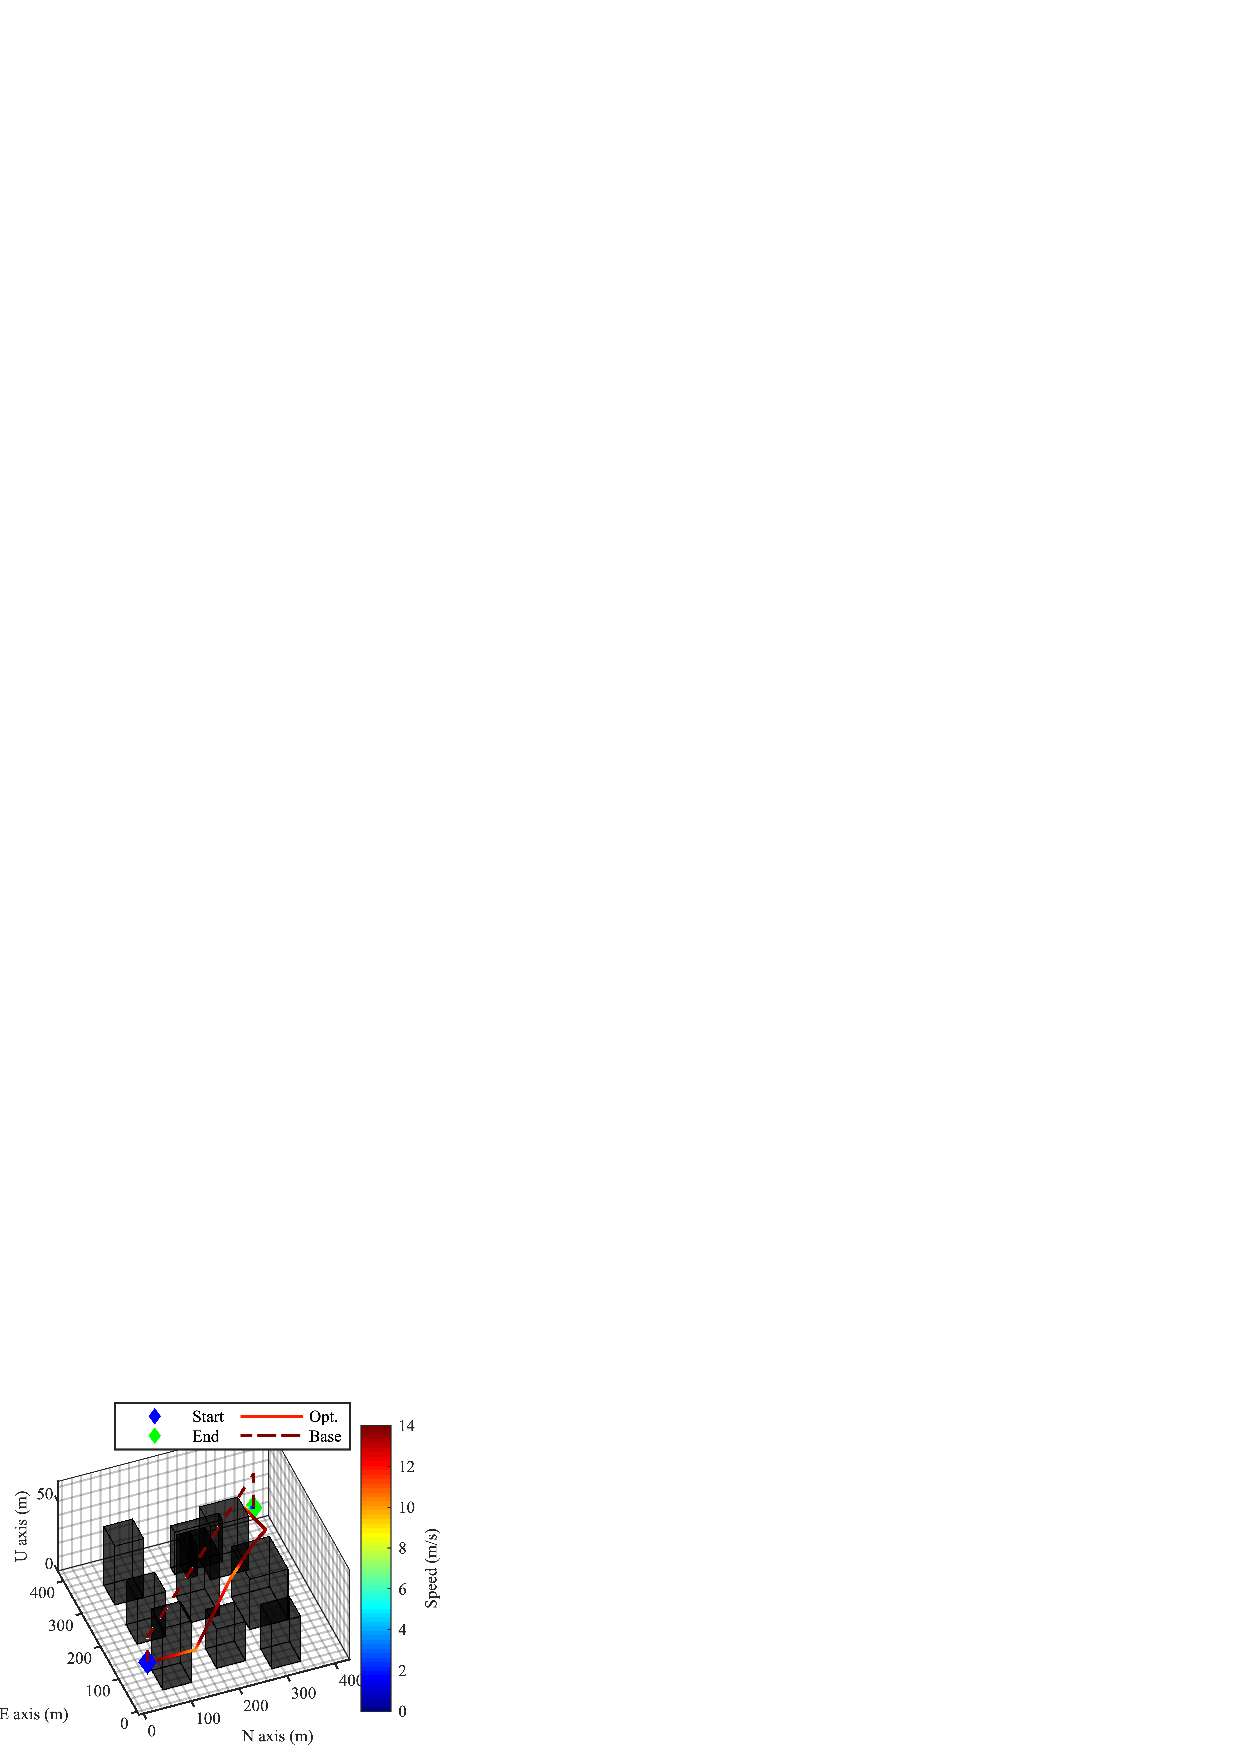
\includegraphics[scale=1.0]{fig13/opt_iso.pdf}}
\qquad
\subfloat[The top view of the baseline and optimized path in the drone flight environment.]{\centering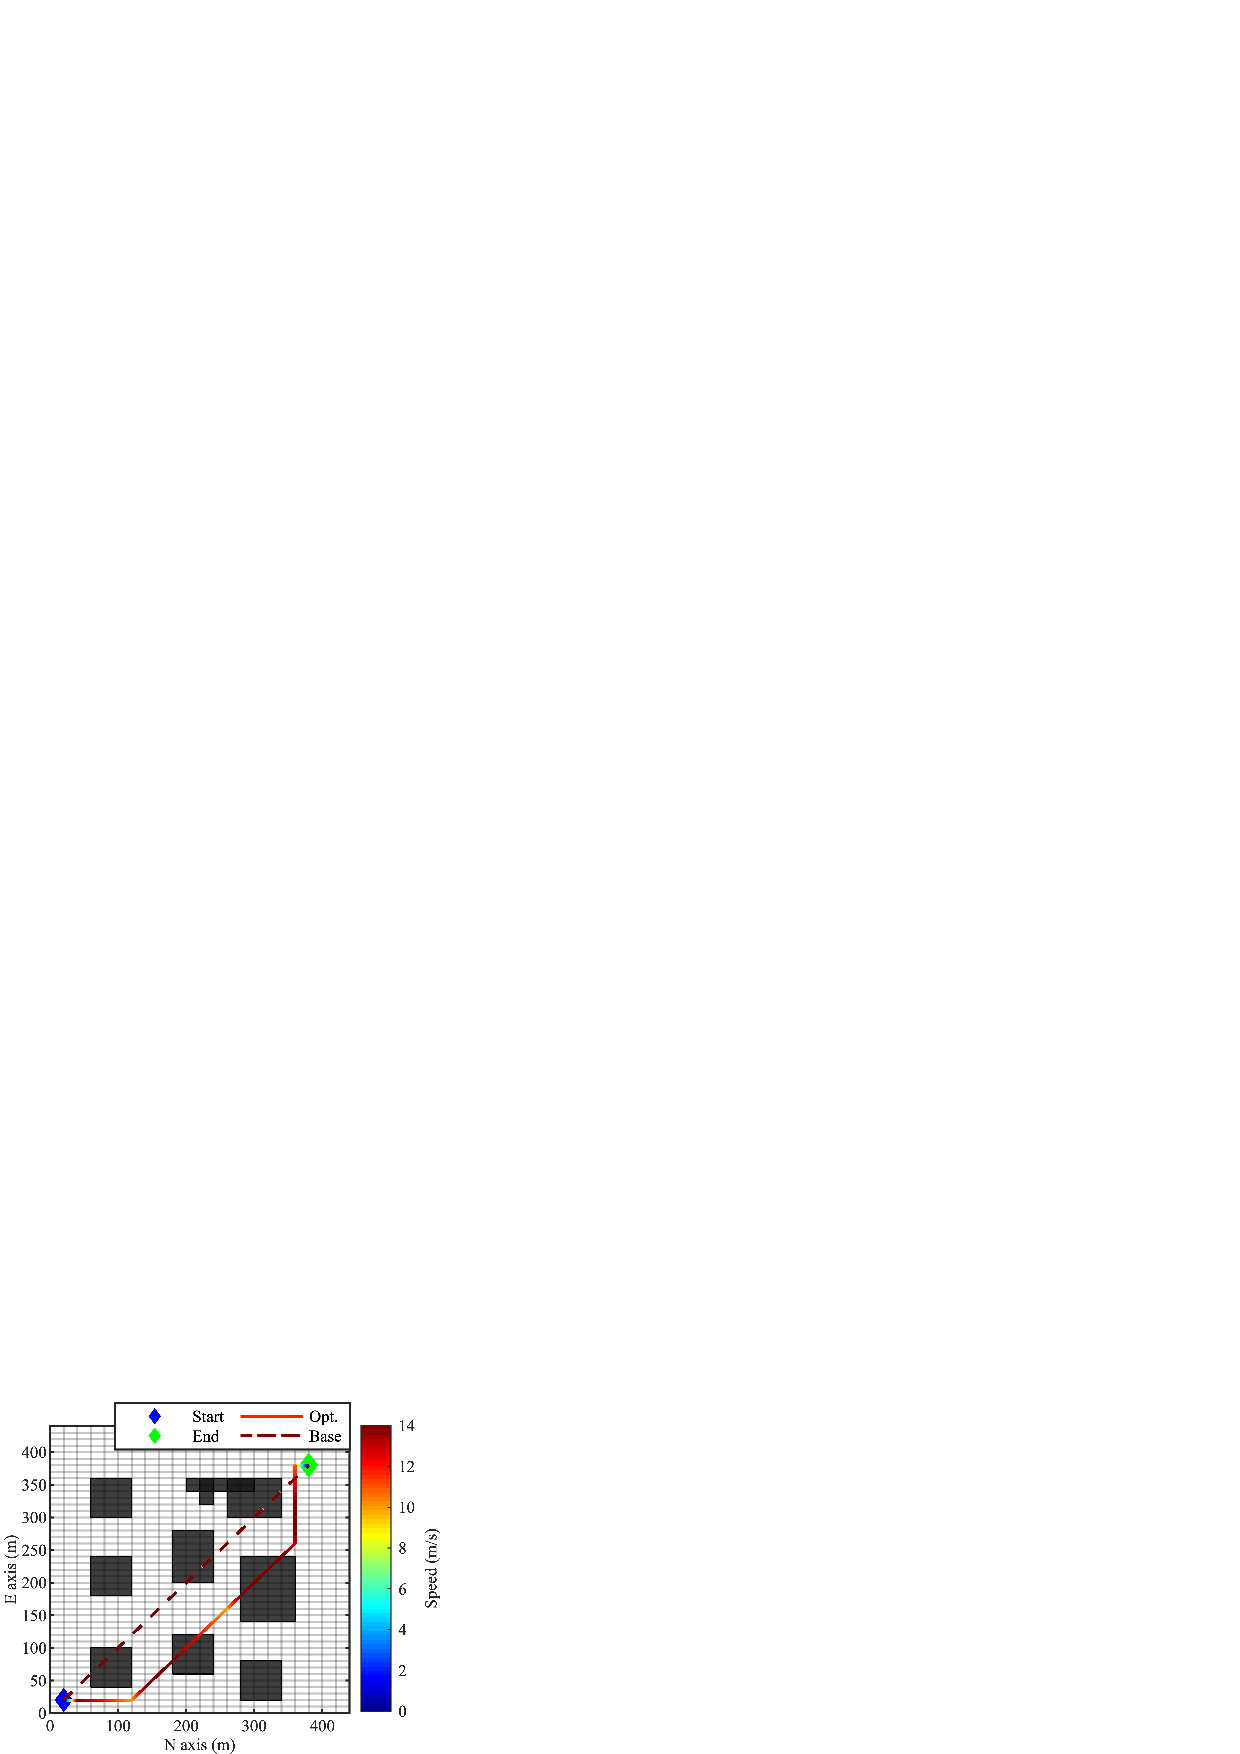
\includegraphics[scale=1.0]{fig13/opt_top.pdf}}
\caption{The minimum energy optimization result of \textcolor{red}{a drone in the operating environment, assuming that there is no wind}.}
\label{fig: opt_environ}
\end{figure}

\begin{figure}[ht]
\fcolorbox{red}{white}{
\centering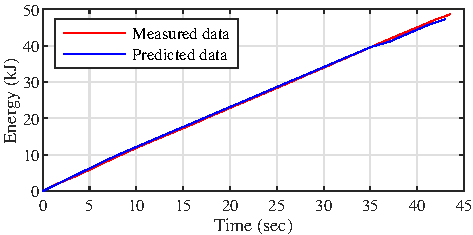
\includegraphics[scale=1.0]{fig14/S_E.pdf}
}
\caption{\textcolor{red}{Comparison of the energy consumption derived by actual flight and simulation of the M600.}}
\label{fig:consumed_energy}
\end{figure}

\begin{figure*}[htp!b]
\begin{mdframed}[linecolor=red]
\centering
%\fcolorbox{red}{white}{
\subfloat[\textcolor{red}{Optimization result of case 1: We assume that there is i) no wind, ii) south-east direction wind, iii) north direction wind.}]{\centering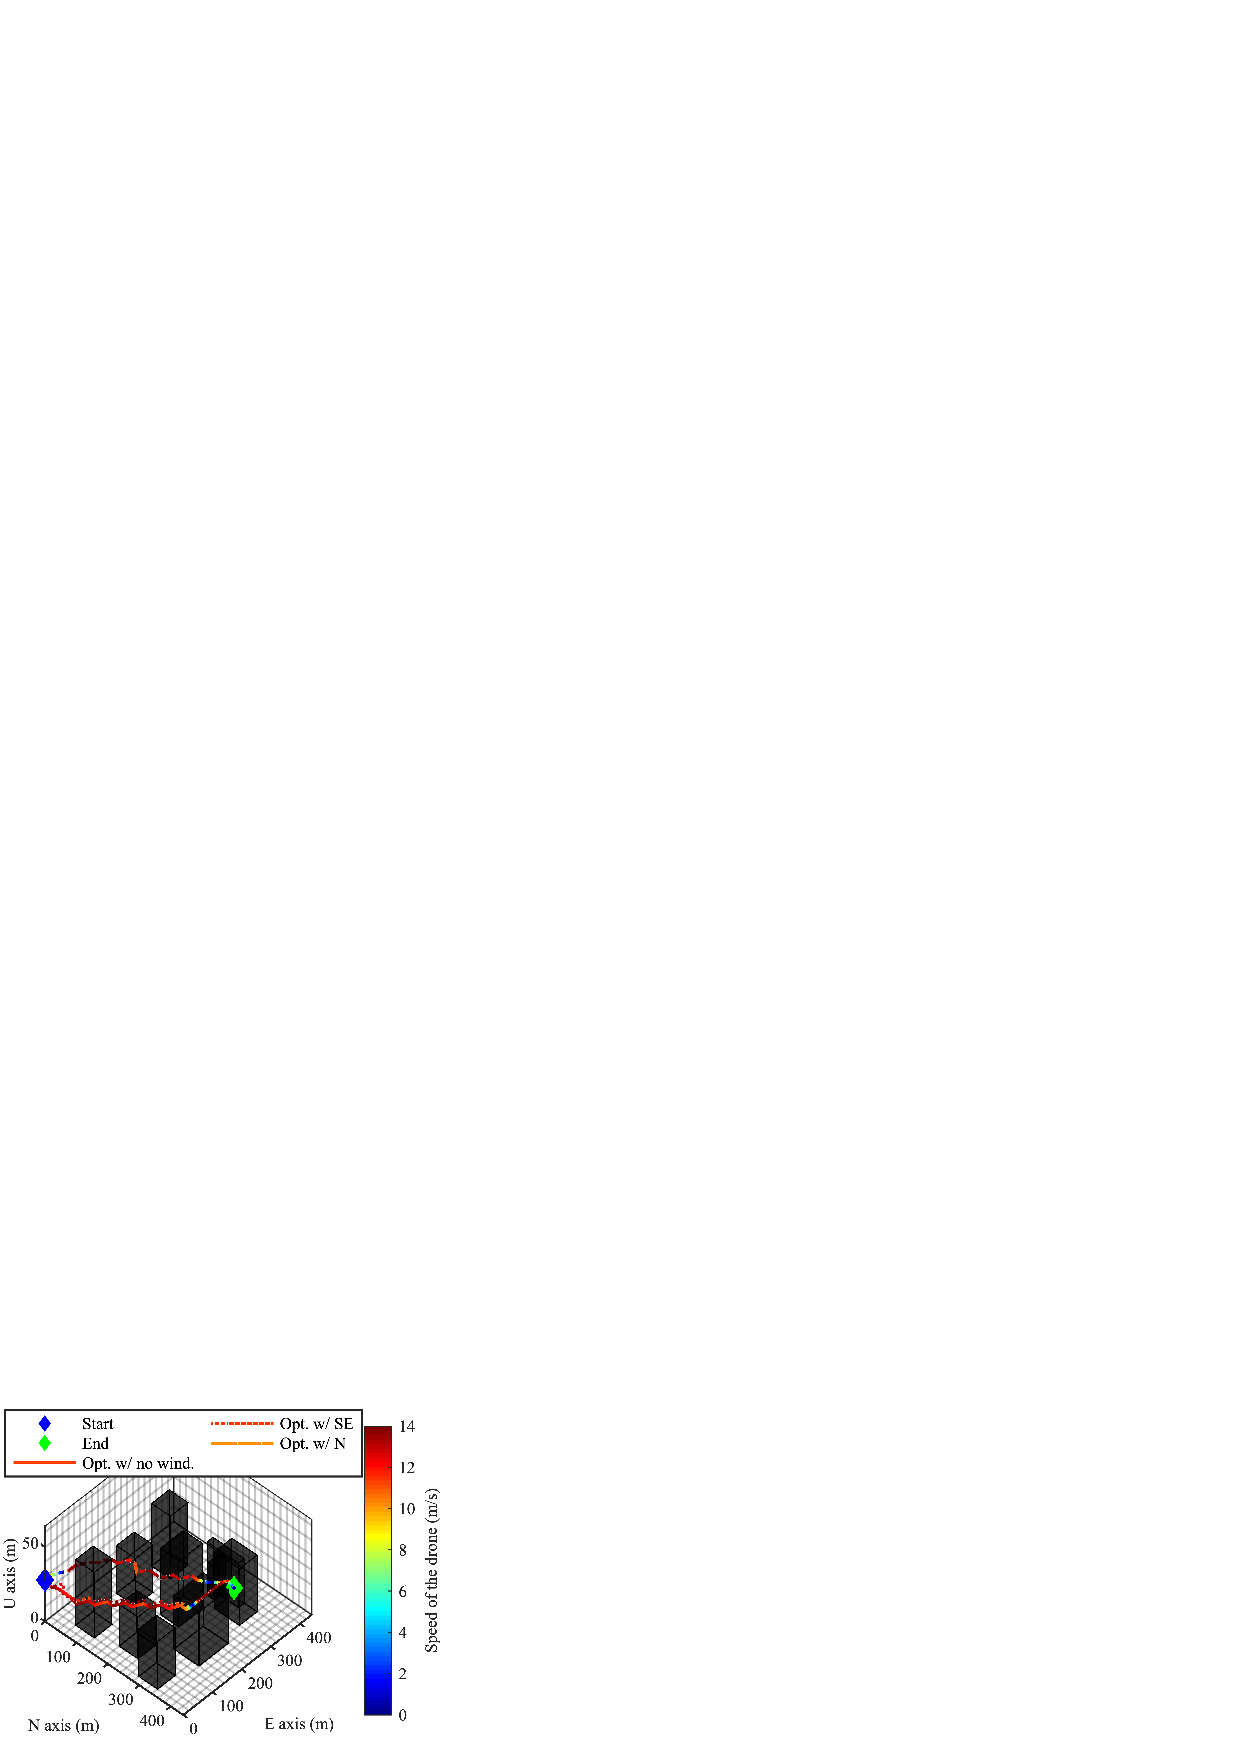
\includegraphics[scale=0.71]{fig15/wind1_iso.pdf}}
\subfloat[The top view of \textcolor{red}{optimized drone path}.]{\centering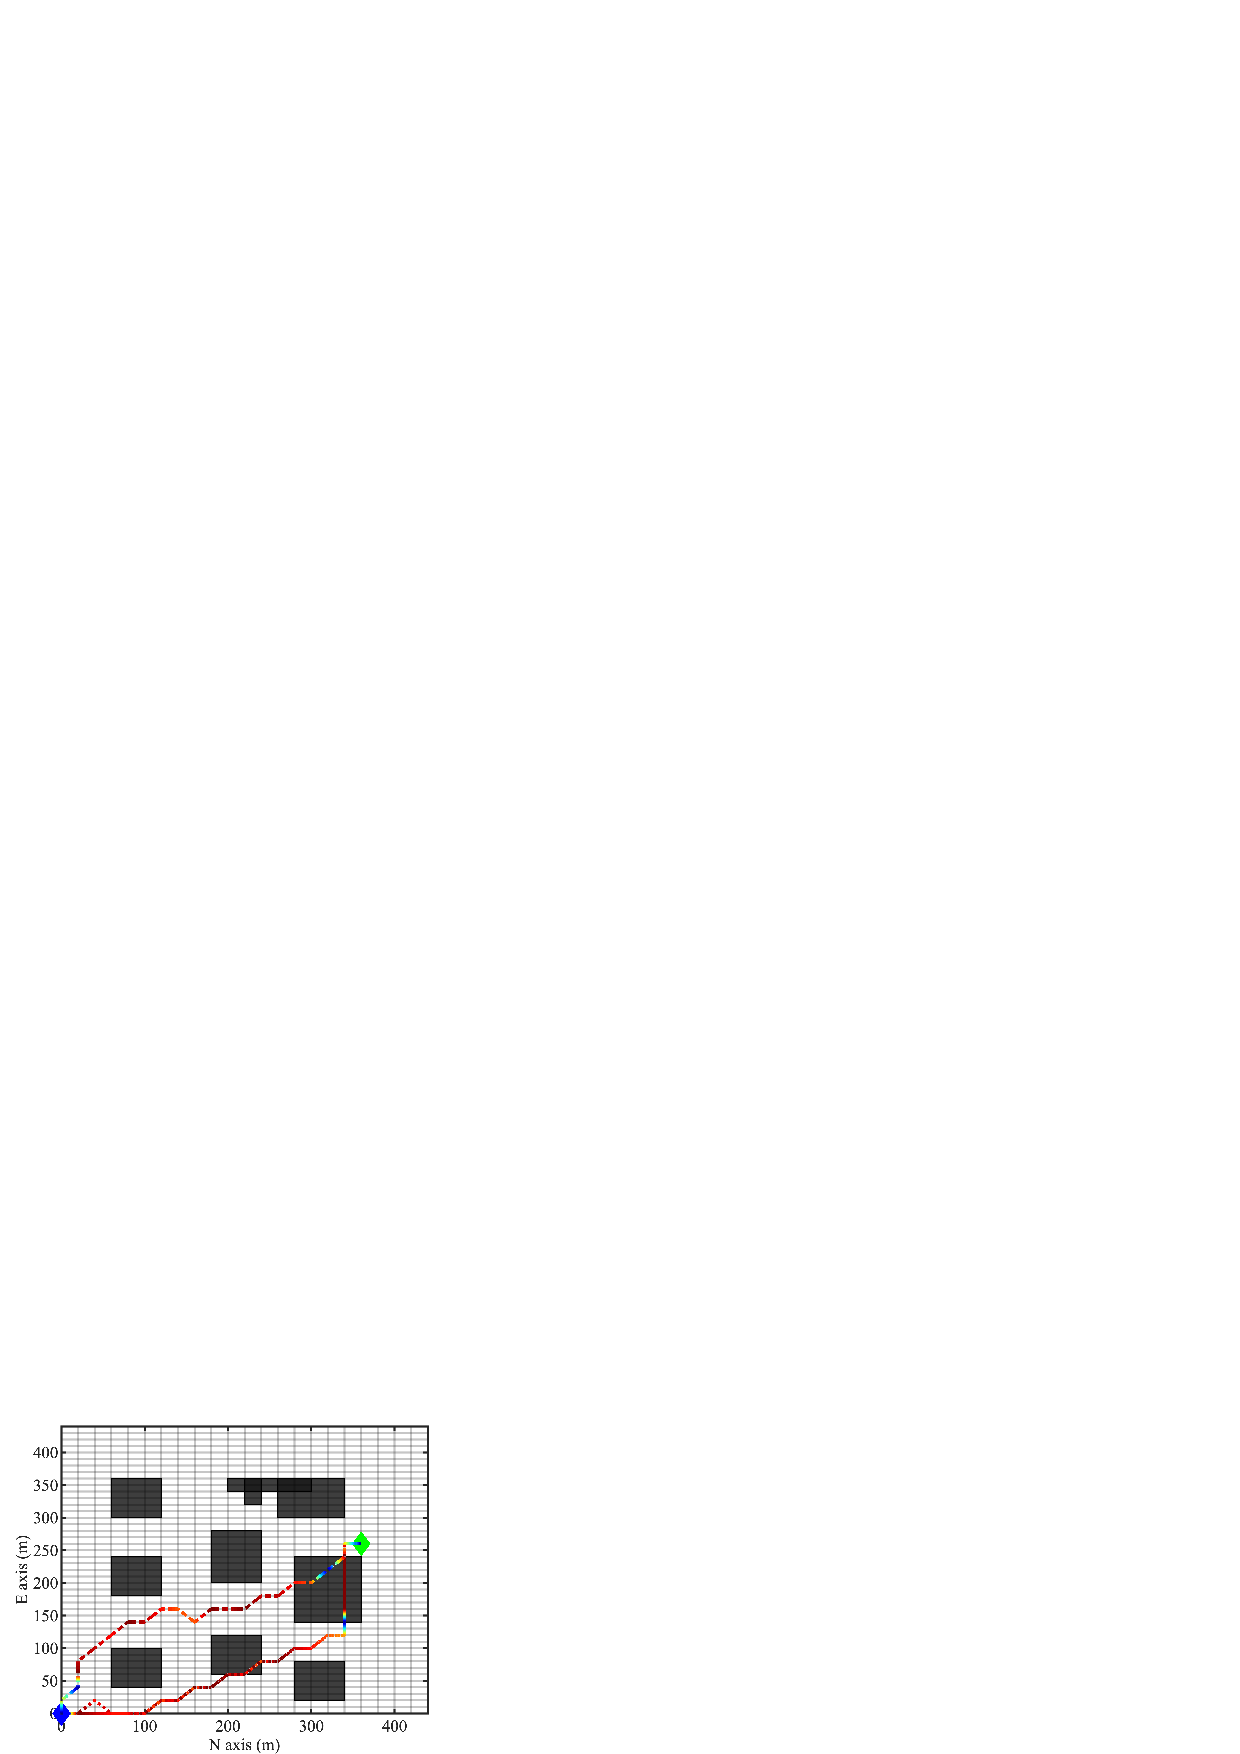
\includegraphics[scale=0.71]{fig15/wind1_top.pdf}}
\subfloat[The side view of \textcolor{red}{optimized drone path}.]{\centering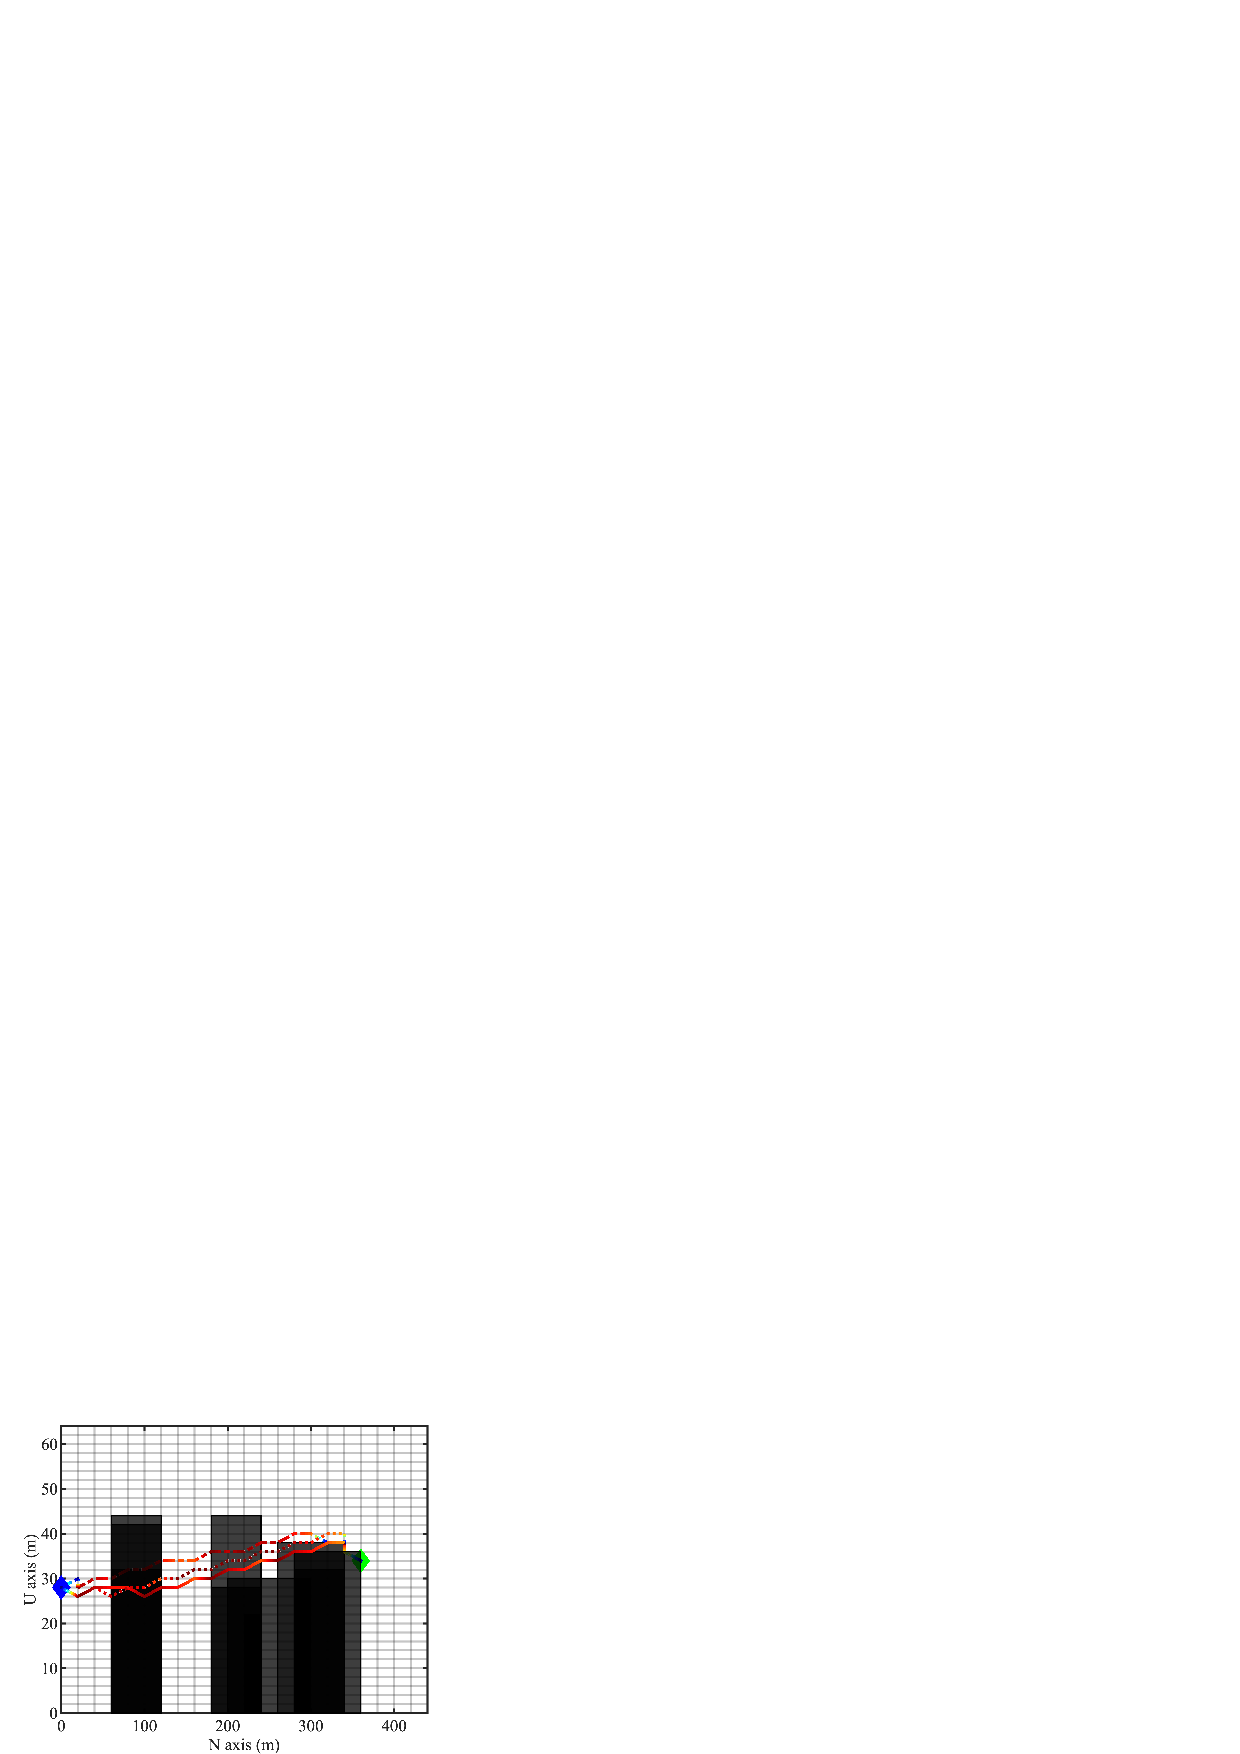
\includegraphics[scale=0.71]{fig15/wind1_side.pdf}}
\qquad
\subfloat[\textcolor{red}{Optimization result of case 2: We assume that there is i) no wind, ii) north-west direction wind, iii) south-east direction wind.} In this figure, we rotate the figure to show the drone path clearly. ]{\centering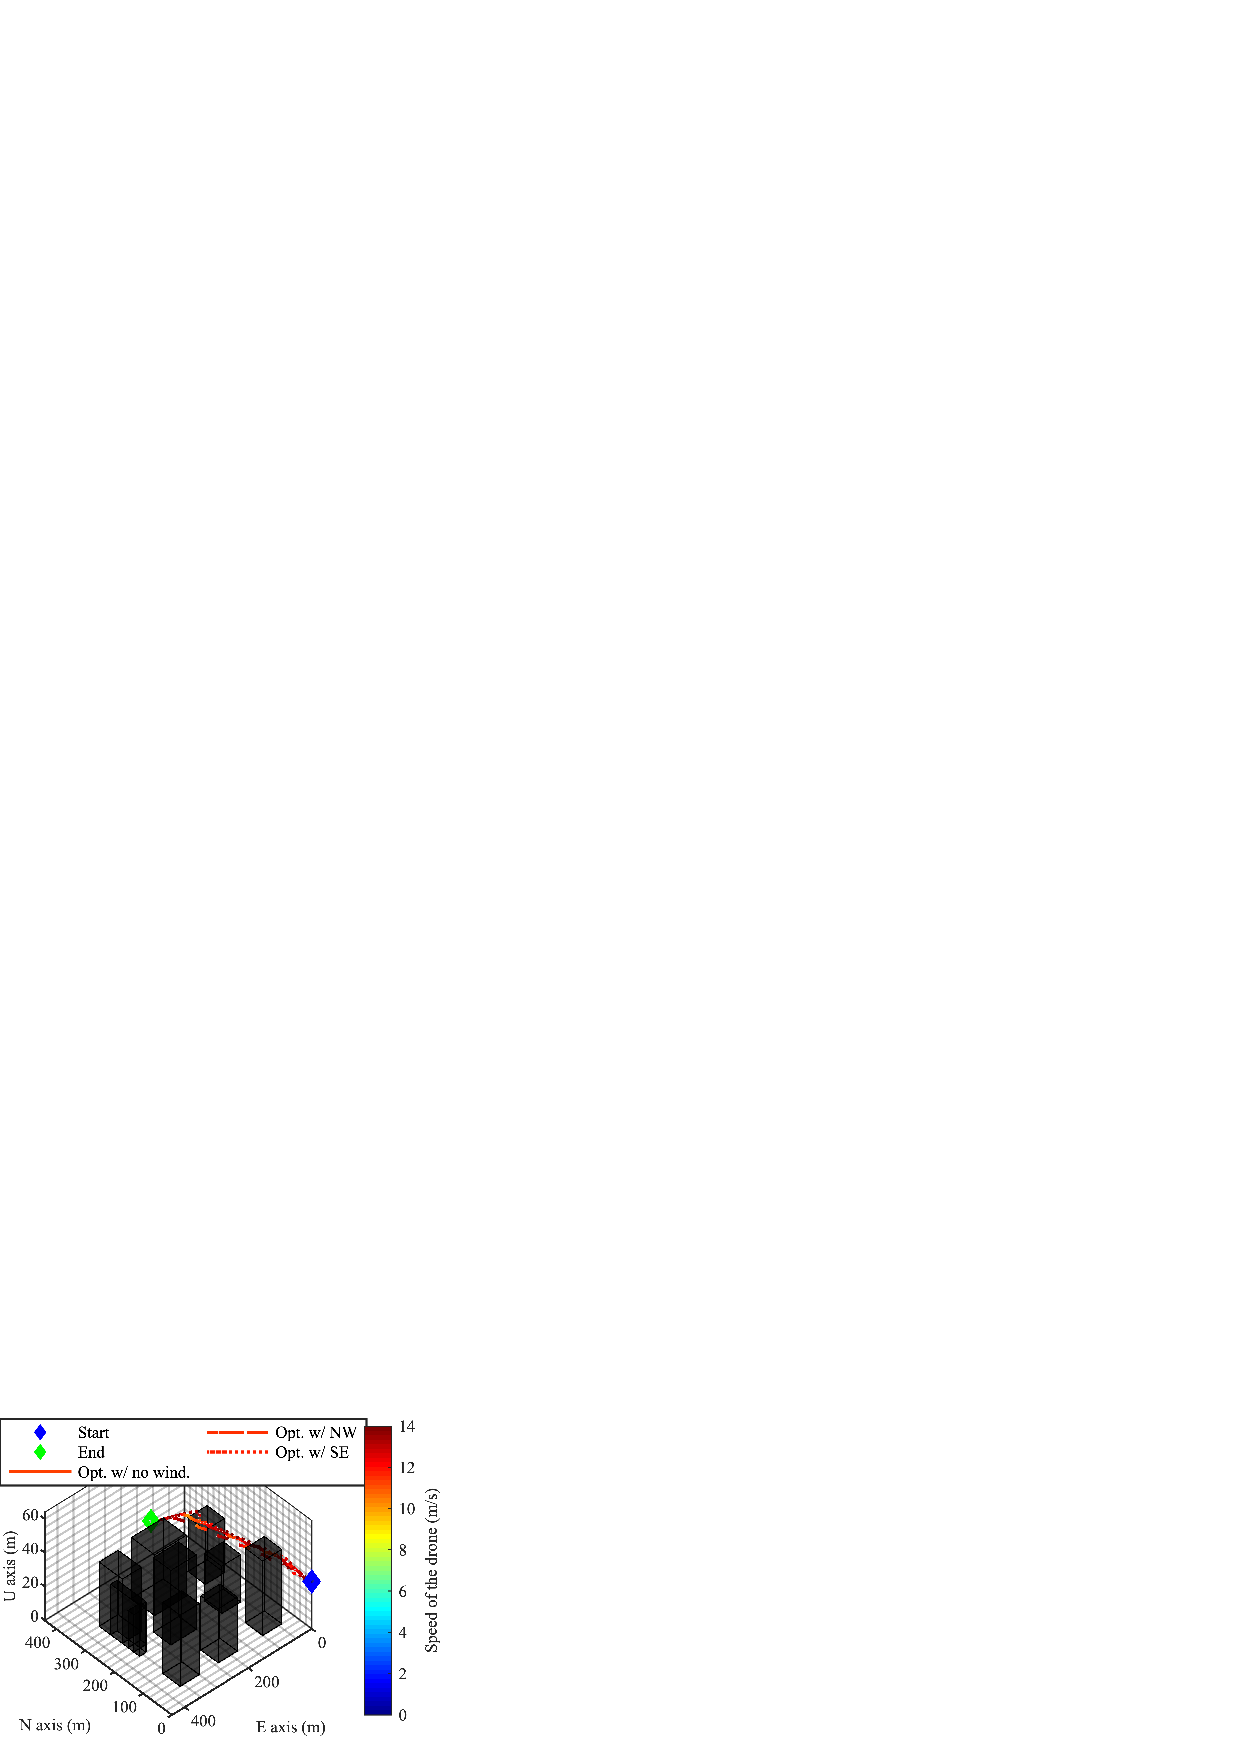
\includegraphics[scale=0.71]{fig15/wind2_iso.pdf}}
\subfloat[The top view of \textcolor{red}{optimized drone path}.]{\centering\includegraphics[scale=0.71]{fig15/wind2_top.pdf}}
\subfloat[The side view of \textcolor{red}{optimized drone path}.]{\centering\includegraphics[scale=0.71]{fig15/wind2_side.pdf}}
\qquad
\subfloat[\textcolor{red}{The discretized north direction wind map.}]{\centering\includegraphics[scale=0.72]{fig15/wind_N.pdf}}
\subfloat[\textcolor{red}{The discretized north-west direction wind map.}]{\centering\includegraphics[scale=0.75]{fig15/wind_NW.pdf}}
\subfloat[\textcolor{red}{The discretized south-east direction wind map.}]{\centering\includegraphics[scale=0.75]{fig15/wind_SE.pdf}}
    \caption{
        \textcolor{red}{Optimization result of two example cases (a-f) considering wind map derived by the inlet velocity with 9~m/s (g-i). 
        The drone travel in the SE direction between the two points that are at different altitudes.}
    }
\label{fig: wind_opt}
\end{mdframed}
\end{figure*}


\noindent The movement velocity of the drone in the two paths is based on the translational lift effect \textcolor{red}{of subsection\,\ref{sub_section:lift}}.
\textcolor{red}{A drone following the} baseline \textcolor{red}{path} maintains the uniform velocity that achieves the minimum energy consumption over the distance. 
\textcolor{red}{The} total power consumption \textcolor{red}{of the drone} from the start point to \textcolor{red}{destination} is 49.78\,kJ.
\textcolor{red}{However, the derived optimal path makes a drone have velocity variations by the path changes to avoid obstacles.} 
The total power consumed by \textcolor{red}{the drone following the} proposed optimal path is 46.1\,kJ, which is 8.4\,\% more efficient than the baseline. 
\textcolor{red}{As the simulation results, the drone following the optimal path saves energy by bypassing a high-level obstacle or overcoming a low-level obstacle in a nearby environment instead of overcoming the highest obstacle in the path.
%Besides, the acceleration and the deceleration occurring in the drastic direction change of drone considerably affect the power consumption of the drone.
We measure the power consumption of the drone during the actual flight to verify the fidelity of the simulation result.
The comparison results of the consumed energy at the simulated flight and actual flight of the drone are presented in Fig.\,\ref{fig:consumed_energy}.}
The drone consumes the energy of 48.8\,kJ through the actual flight \textcolor{red}{using a real drone}, and the proposed simulation predicts the energy consumption of 46.1\,kJ.
There is a 5.54\,\% difference between the energy consumption predicted by the simulator and the energy consumed by the real flight.
The validation through the actual flight of the drone shows that the energy consumption deduced by the proposed simulation and the energy consumption of the real flight are not significantly different.



\subsection{\textcolor{red}{Optimization results affected by the external forces}}

\begin{table*}[!h]
\caption{\textcolor{red}{Comparison of the energy consumption between the baseline and the optimal path affected by wind in each case.}}
\centering
\fcolorbox{red}{white}{
\label{tab: opt.result}
%\resizebox{\textwidth}{!}{%
\textcolor{red}{
\begin{tabular}{|c|c|c|c|c|c|c|}
\hline
\multirow{2}{*}{} & \multirow{2}{*}{Wind map} & \multicolumn{2}{c|}{Energy consumption (kJ)} & \multicolumn{2}{c|}{Travel time (sec)} & \multirow{2}{*}{Saved energy (\%)} \\ \cline{3-6}
                        &            & Baseline & Optimal path & Baseline               & Optimal path &      \\ \hline
\multirow{2}{*}{Case 1.} & Fig.~\ref{fig: wind_opt}~(i) & 38.1     & 36.2         & \multirow{2}{*}{44.10} & 40.84        & 5.3 \\ \cline{2-4} \cline{6-7} 
                        & Fig.~\ref{fig: wind_opt}~(g) & 46.3     & 45.4         &                        & 46.53        & 1.8  \\ \hline
\multirow{2}{*}{Case 2.} & Fig.~\ref{fig: wind_opt}~(i) & 44.7     & 43.9         & \multirow{2}{*}{53.58} & 50.68        & 1.9  \\ \cline{2-4} \cline{6-7} 
                        & Fig.~\ref{fig: wind_opt}~(h) & 45.7     & 45.4         &                        & 52.33        & 0.7  \\ \hline
\end{tabular}%
}
}
%}
\end{table*}

\textcolor{red}{In this section, we present} the path that \textcolor{red}{requires} the least energy in the environment where the wind effect exists, and \textcolor{red}{compare} the energy consumption with the previous optimized path \textcolor{red}{that does not consider wind effects}.
\textcolor{red}{We present two examples of flight missions and three wind maps used in Fig.\,\ref{fig: wind_opt}.
First, we present the two missions in Figs.\,\ref{fig: wind_opt}(a) and (d) as the isometric view.
The baseline of each case is a derived path assumed that it is not affected by wind as Fig.\,\ref{fig: opt_environ}. %but we calculate the energy consumption of these paths by applying the wind direction and speed of wind maps.
} 
The two figures next to each mission are \textcolor{red}{the} side-view and top-view \textcolor{red}{paths} to identify the changes in the path and the difference in elevation.  
\textcolor{red}{We also present three wind maps in Figs.\,\ref{fig: wind_opt} (g), (h), and (i), which are used as parameters to reveal the influence of wind.
The two cases differ in the location and height of the destination. Also, we use two wind maps for each case to check the change in path due to wind.
For Case 1, we apply the wind maps of the north and south-east direction.
When the south-east wind exists, the baseline and the optimized path are similar, but there is a difference in the height between paths. 
The optimized path consumes a total of 36.2\,kJ of energy, which is 5.3\,\% more efficient than a baseline that consumes the energy of 38.1\,kJ.
On the other hand, when the north wind exists, the optimized path is much different from a baseline even it shows not much different energy consumption.
The optimized path consumes a total of 45.4\,kJ of energy, which is 1.8\,\% more efficient than a baseline that consumes the energy of 46.3\,kJ.
%We confirm that all paths are similar, but energy differences occur due to the difference in altitude of each path.
In Case 2, we apply the wind maps of the north-west and south-east direction.
When the south-east wind exists, the optimized path consumes a total of 43.9\,kJ of energy, which is 1.9\,\% more efficient than the baseline that consumes the energy of 44.7\,kJ.
When the north-west wind exists, the optimized path consumes a total of 45.4\,kJ of energy, which is 0.7\,\% more efficient than the baseline that consumes the energy of 45.7\,kJ.}
\textcolor{red}{As a result}, we present \textcolor{red}{our} optimization results as Table\,\ref{tab: opt.result} that \textcolor{red}{contains comparisons of the energy consumption between the baseline and the optimal path and the time taking when the drone travels along paths.
Especially, Case 1 shows an impressive result. 
We aim that find a way to reduce the drone's energy consumption by optimizing the path to the influence of the external environment without significant hardware improvements, and the result shows that even if the drone flies for about 3 seconds longer than the baseline, the optimal path consumes less energy than the baseline.}












%요까지 다 봤음. Jaemin.
\section{Conclusions}

In this paper, we present a systematic framework for optimizing the total operating cost of drones, including accurate power consumption models and optimization methods.
We start from a demonstration that the data provided by the factory onboard power measurement feature of even top-of-the-line commercial drones is highly inaccurate by comparing it with standard equipment. 
This motivates that the power consumption models shown in the previous work may have generated improper predictions compared with the actual power consumption due to the inaccuracy in the measured data.
We implement an accurate in-house onboard power measurement \textcolor{red}{system} and collect dozens of hours of power measurement data with other \textcolor{red}{flight} data. 
Based on the power data, we propose an accurate power consumption model with the deep neural networks. 
The proposed power consumption model exhibits error within 10\,\% compared with a high standard precision data acquisition device. 
%The primary benefit of the proposed model is such that i) the model inputs are simple physics parameters of the drone and external factors affecting power consumption thus it can be easily plugged in a various existing optimization framework, and ii) the characterization process is not dependent on the aerodynamics of a particular drone. 
Then, we present how to find the optimized path by using a dynamic programming algorithm with the proposed accurate power consumption model and our heuristics.
Finally, we demonstrate example\textcolor{red}{s} of finding an energy-efficient path.
The optimal path is derived by \textcolor{red}{considering} the wind effects that are generally difficult to consider, and the optimal path \textcolor{red}{shows gain up to 5.27\,\% considering the wind}.










\section*{Acknowledgment}
This work was supported by the National Research Foundation of Korea (NRF-2018R1A2B3007894) and the 2019 Research Fund of Myongji University. 

\bibliographystyle{unsrt}%Used BibTeX style is unsrt
\bibliography{reference}

\begin{IEEEbiography}[{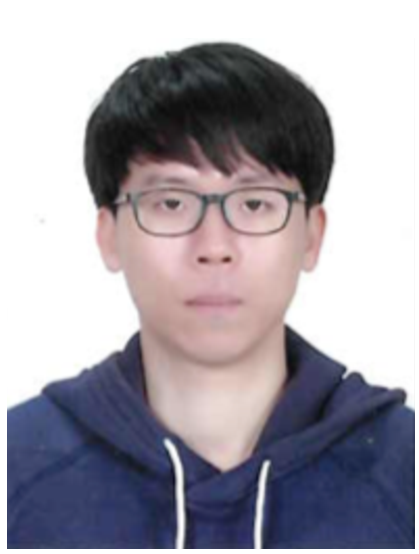
\includegraphics[width=1in,height=1.25in,clip,keepaspectratio]{./bio/dooyoung}}]{Dooyoung Hong}
(S'18) received the B.S. degree in mechanical engineering from Korea University of Technology and Education, Cheonan, Korea in 2017 and received the M.S. degree in the robotics program from Korea Advanced Institute of Science and Technology, Daejeon, Korea in 2019. He is currently pursuing Ph.D. degree in the robotics program, Korea Advanced Institute of Science and Technology. His research interests include low-power embedded system design, and AI based optimization.
\end{IEEEbiography}

\begin{IEEEbiography}[{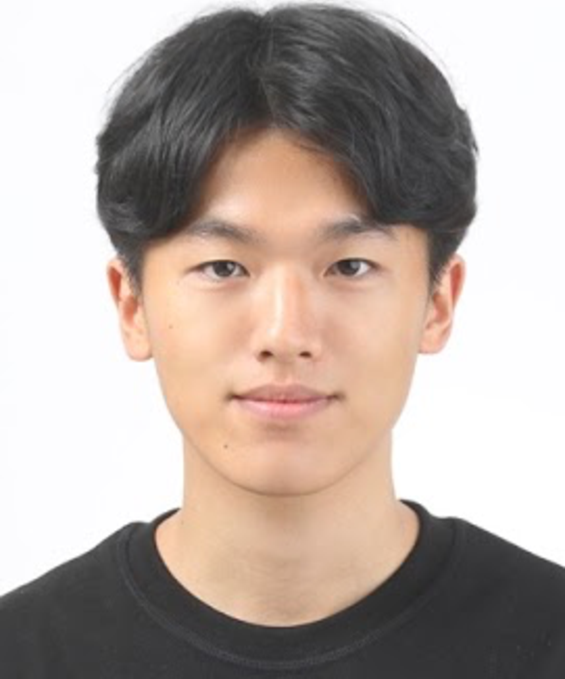
\includegraphics[width=1in,height=1.25in,clip,keepaspectratio]{./bio/seonhoon}}]{Seonhoon Lee}
(S'18) received the B.S. degree in electrical engineering from Konkuk University, Seoul, Korea in 2018. He is currently pursuing a master’s degree in the school of electrical engineering, Korea Advanced Institute of Science and Technology. His research interests include low-power embedded system, cyber-physical system, and deep learning.
\end{IEEEbiography}

\begin{IEEEbiography}[{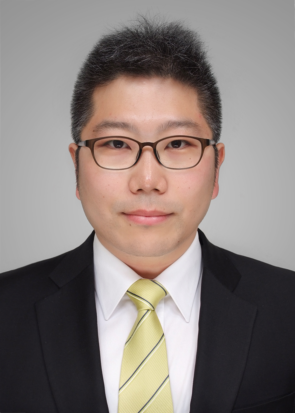
\includegraphics[width=1in,height=1.25in,clip,keepaspectratio]{./bio/jaemin}}]{Jaemin Kim}
(S'13 M'18) received the B.S. degree in computer science engineering and the M.S. and Ph.D. degrees in computer science and electrical engineering from Seoul National University, Seoul, Korea, in 2005, 2007, and 2018 respectively. He is currently an assistant professor at the department of electronics engineering, Myongji University. His research interests include low-power embedded system design, electrical energy storage system, and energy soruce reconfiguration system.
\end{IEEEbiography}

\begin{IEEEbiography}[{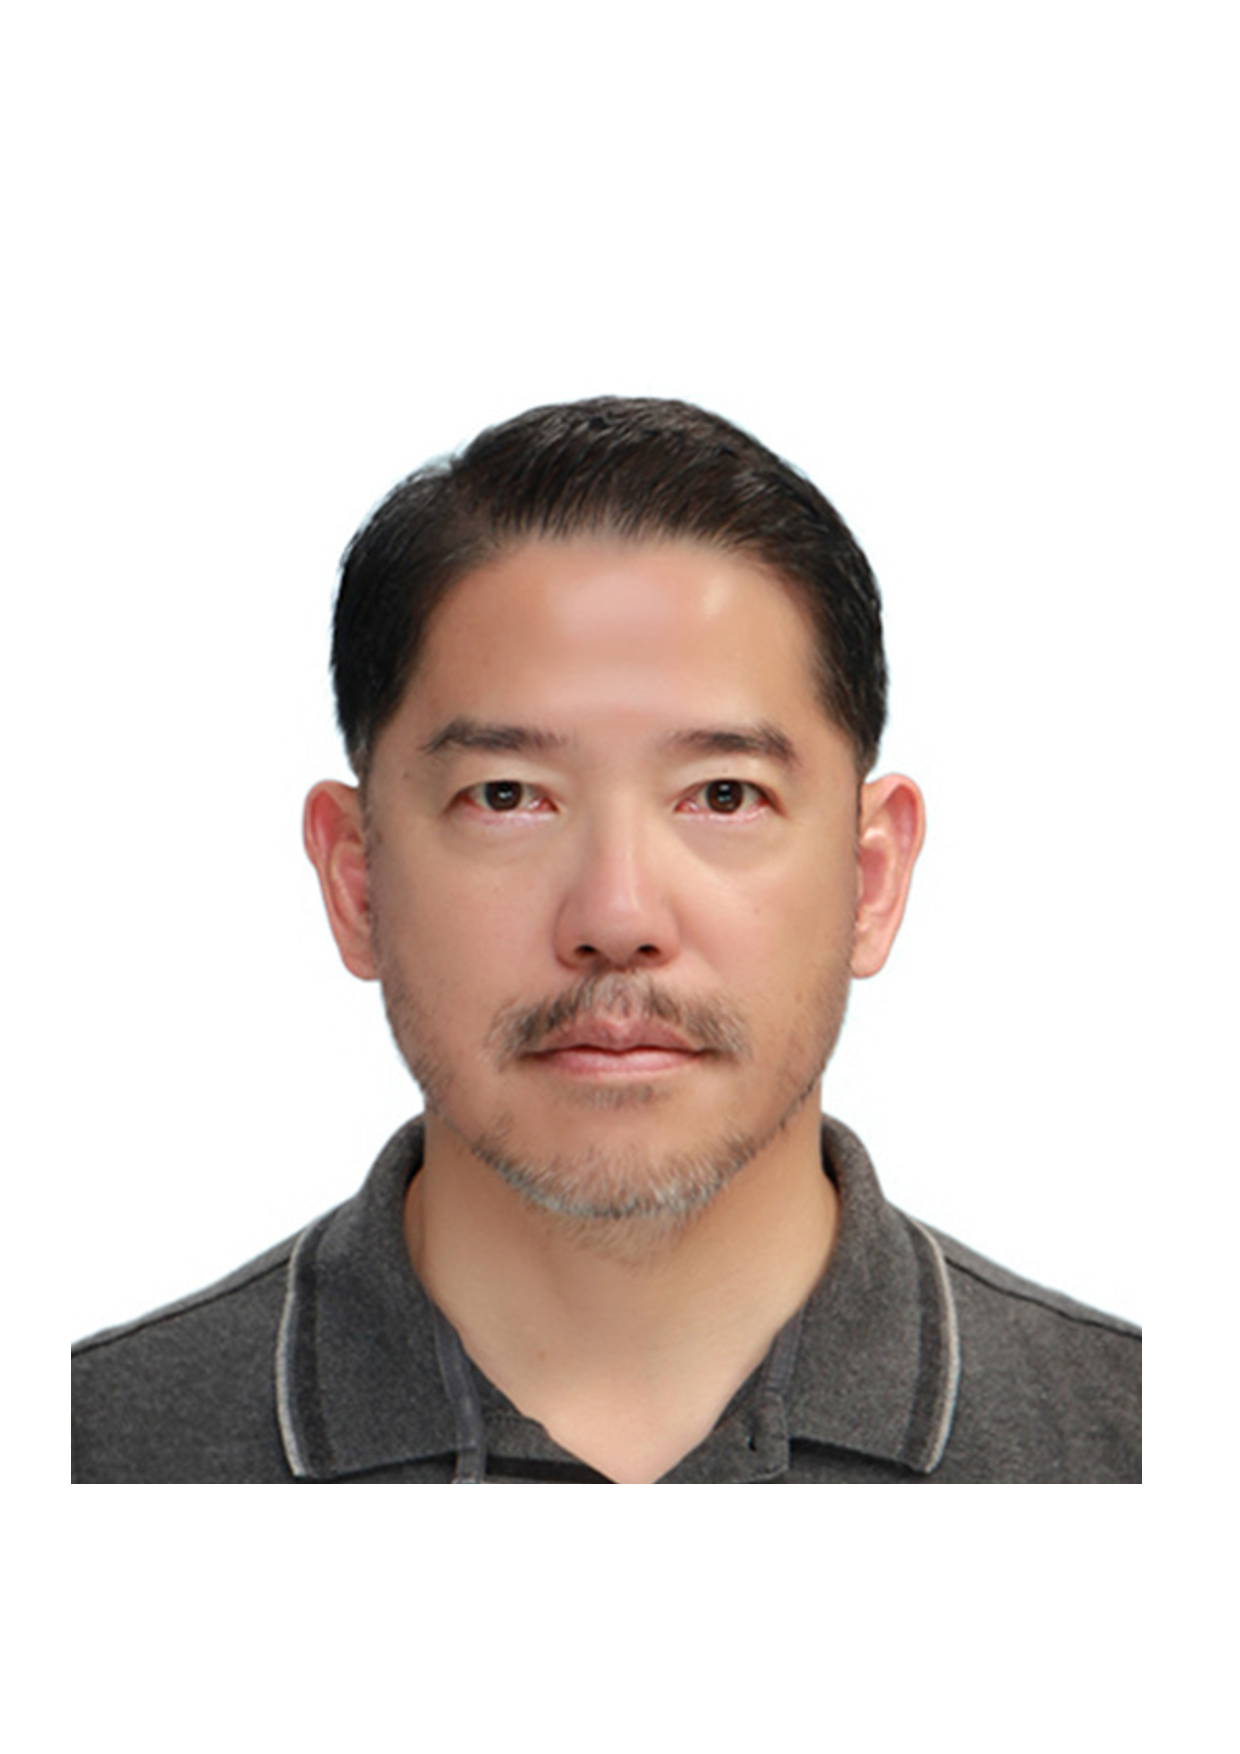
\includegraphics[width=1in,height=1.25in,clip,keepaspectratio]{./bio/naehyuck}}]{Naehyuck Chang}
(F’12) received the B.S., M.S., and Ph.D. degrees from the Department of Control and Instrumentation, Seoul National University, Seoul, South Korea, in 1989, 1992, and 1996, respectively.
From 1997 to 2014, he was at the Department of Computer Science and Engineering, Seoul National University. In 2005, he was a Research Professor at LG Yonam Foundation, Seoul. From 2011 to 2013, he was a Vice Dean of the College of Engineering, Seoul National University. Since 2014, he has been
a Full Professor at the Department of Electrical Engineering, Korea Advanced Institute of Science and Technology, Daejeon, South Korea. He is the Co-Founder of EMVcon, Inc., Irvine CA, USA. His current research interests include low-power cyber-physical systems and design automation of things, such as systematic design and optimization of energy storage systems, electric vehicles, drones, energy harvesting, and so on.
Dr. Chang is a Fellow of the Association for Computing Machinery (ACM) for his contributions to low-power systems. 
\begin{comment}%Accept되고 나서 원복
He served as the Chair and the Past Chair for ACM Special Interest Group on Design Automation. He was the TPC Co-Chair of DAC 2016, ASP-DAC 2015, ICCD 2014, CODES+ISSS 2012, ISLPED 2009, and so on, and the General Co-Chair of VLSI-SoC 2015, ICCD 2015 and 2014, ISLPED 2011, and so on. He was a recipient of the 2014 ISLPED Best Paper Award, the 2011 SAE Vincent Bendix Automotive Electronics Engineering Award, the 2011 Sinyang Academic Award, the 2009 IEEE SSCS International SoC Design Conference Seoul Chapter Award, and several ISLPED Low-Power Design Contest Awards in 2002, 2003, 2004, 2007, 2012, 2014, and 2017. He is the Editor-in- Chief of the ACM Transactions on Design Automation of Electronics Systems and serves(ed) as an Associated Editor of the IEEE TRANSACTIONS ON VERY LARGE SCALE INTEGRATION, the IEEE TRANSACTIONS ON COMPUTER AIDED DESIGN OF INTEGRATED CIRCUITS AND SYSTEMS, the ACM Transactions on Embedded Computing Systems, IEEE EMBEDDED SYSTEMS LETTERS, the IEEE TRANSACTIONS ON CIRCUITS AND SYSTEMS–PART I: REGULAR PAPERS, and so on.
\end{comment}
\end{IEEEbiography}


\end{document}
